\documentclass[noframe,twoside]{ncuthesisCJK} 
\usepackage{mathptmx}
\usepackage{makeidx}
\usepackage{layout}
\dept{資\quad訊\quad工\quad程\quad學\quad系}
\degree{碩\quad士\quad}
\title{透過網頁瀏覽紀錄預測使用者之個人資訊與性格特質}
\subtitle{Predicting Users' Demographic Information and Personality Through Browsing History}
%\subtitle{}=空白
\author{連丞宥}
\mprof{陳弘軒\hspace{2.3mm}博士}
\degreedate{中~華~民~國\quad一百零七年\quad六月}
 


\def\XeLaTeX{Xe\LaTeX}  % Only in CJK 
%\input{mypreamble}             % 自訂巨集多 收起來
                                 % 自訂巨集少 直接寫出
                                 
\makeindex                       % 告訴\LaTeX要做索引
\begin{document}                 % 宣告結束   本文開始
\begin{CJK}{UTF8}{bkai}          %----------------------
\CJKhorz
\fontsize{12pt}{24pt}\selectfont % 可調間距以便閱讀%
\pagenumbering{alph}             % to cheat latex
\maketitle                       % 論文封面
\setboolean{printcopyright}{true}
%\addtocontents{toc}{~\hfill\textbf{頁次}\par}
%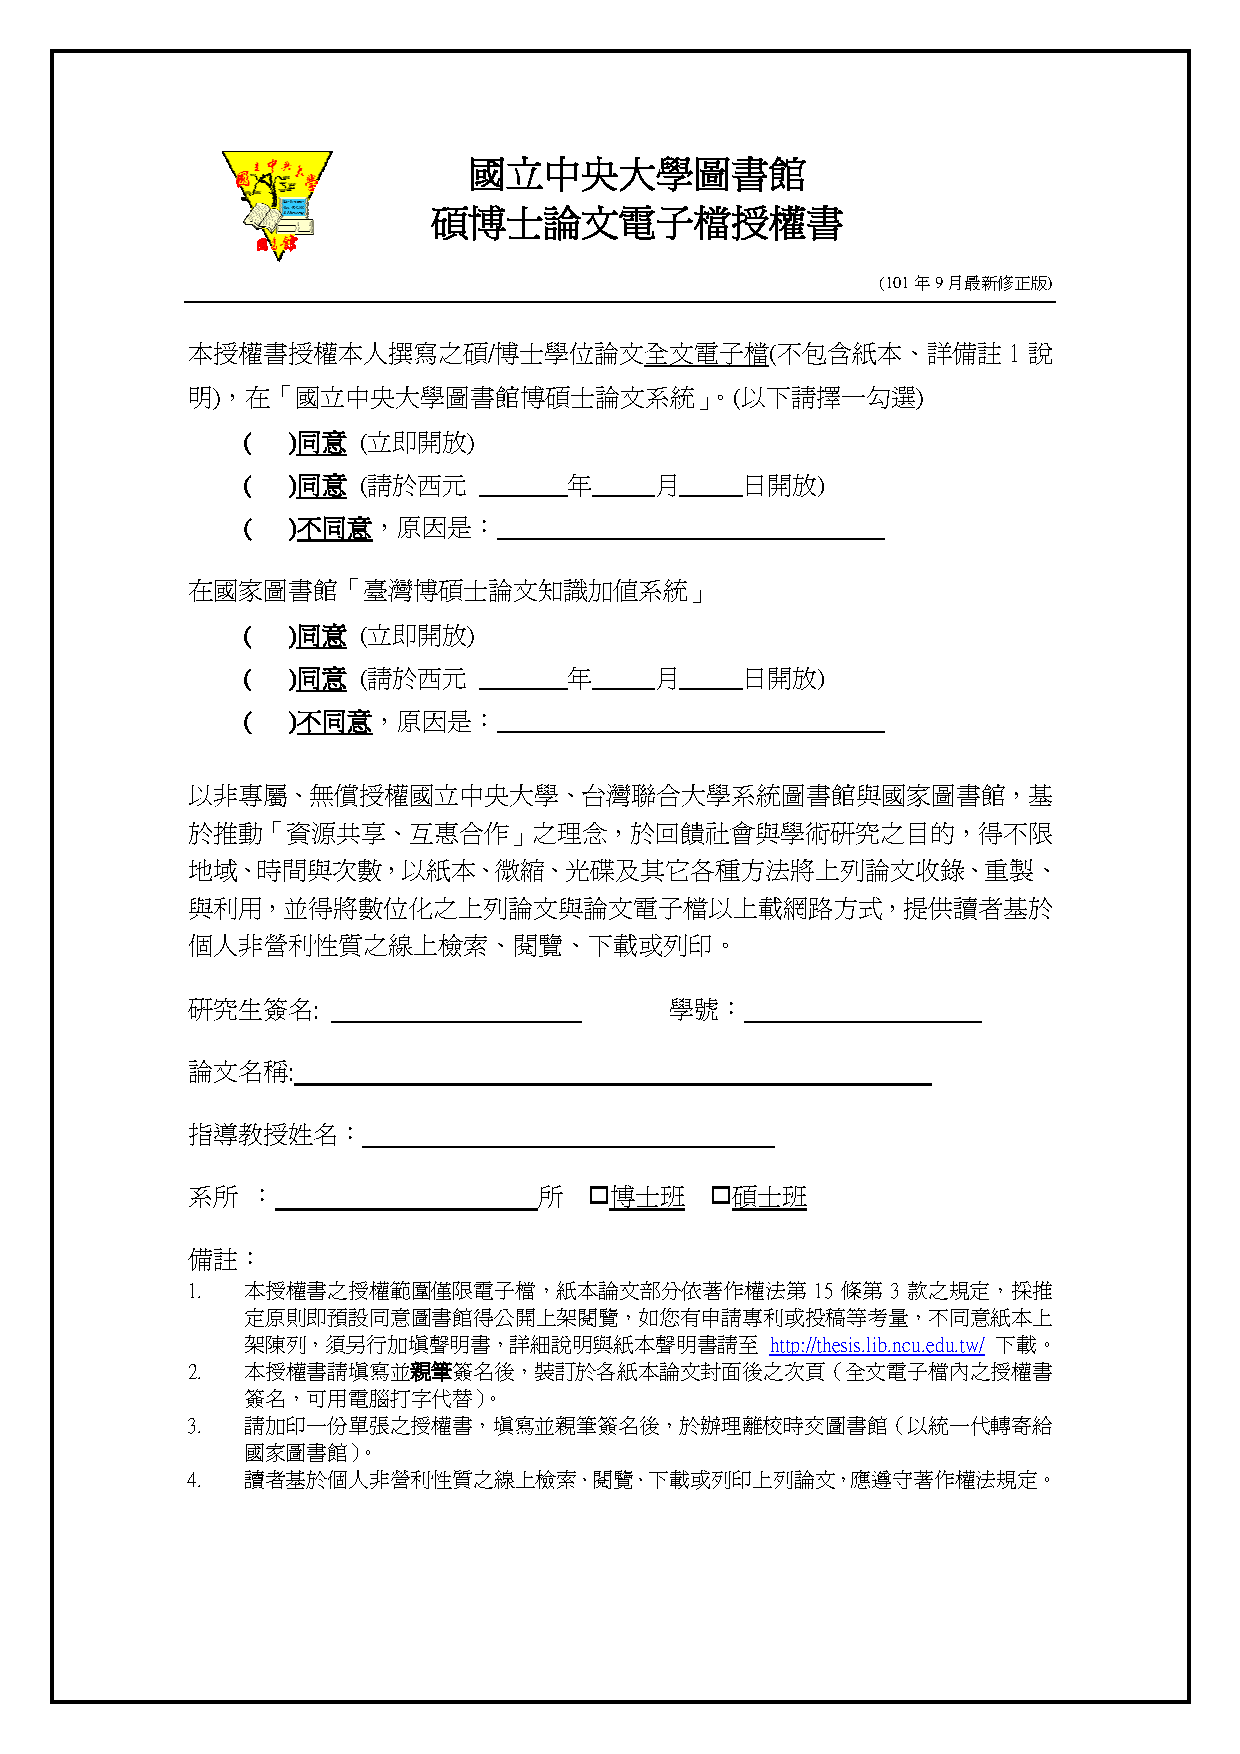
\includepdf[pages=-,scale=0.9]{myfile.pdf} % 插入其他表格
                                 % \frontmatter
\pagenumbering{roman}            % 羅馬數字編頁
\begin{abstractcn}
%\index{ncuthesis 環境!abstractcn}

瀏覽網頁所留下的歷史紀錄能夠描述出使用者瀏覽偏好,因此網頁瀏覽紀錄已經成為了解使用者相關資訊的最佳方式之一。近年來藉由分析使用者瀏覽紀錄並進行個人化商品、廣告推薦的應用逐漸增加,其中影響推薦結果準確度之關鍵在於對使用者相關資訊之掌握度,如果能夠藉由分析網頁瀏覽紀錄來獲得使用者的個人資訊與人格特質將能夠提升推薦系統之效能。\par

本篇論文將 600 位使用者之網頁瀏覽紀錄進行分析並找出較具有代表性的使用者特徵,藉由此使用者特徵搭配分群結合監督式學習方法預測出使用者之性別、年齡、感情狀態與大六性格特質分數,並在準確度上皆有良好的表現。同時也拓展了使用者行為分析的視野,當藉由網頁瀏覽紀錄預測使用者相關資訊時,將不再侷限於個人資訊的預測,而是能夠更加深入了解使用者的個性。\\
 \\
{\bf 關鍵字:}監督式學習、分群、大六性格特質分數

\end{abstractcn}             % 中文摘要 abstractcn環境
\begin{abstracten}
%\index{ncuthesis 環境!abstracten}
\hspace*{8mm} Analyzing an individual’s Internet browsing history is one method of revealing the information about that person; for example, it reveals his/her preference for browsing websites. Analyzing browsing histories has become an increasingly common method for recommending advertisements that may serve individuals’ needs. The accuracy of advertisement recommendations depends on the understanding of a user’s information; thus, a recommender system will be more effective if it can analyze browsing histories to identify users’ demographic information and personalities.\par

This study examined the website browsing histories of 600 users to identify representative user features, which were subsequently analyzed through supervised learning with clustering to make predictions about the users in terms of gender, age, relationship statuses, and big six personality scores. The proposed method enhances the accuracy of the supervised prediction model and broadens the scope of user behavior analyses; particularly, in predicting users’ demographic information, this proposed method clarifies users’ personalities in further depths.\\
\\
{\bf Keyword: }Supervised learning, Clustering, Big-six personality
\end{abstracten} 

             % 英文摘要 abstracten
\clearpage
\phantomsection\addcontentsline{toc}{chapter}{目錄}
\tableofcontents                 % toc
\clearpage
\phantomsection\addcontentsline{toc}{chapter}{圖目錄}
\renewcommand{\numberline}[1]{圖~#1\hspace*{1em}}%圖目錄
\listoffigures                   % lof
\clearpage
\renewcommand{\numberline}[1]{表~#1\hspace*{1em}}%表目錄
\phantomsection\addcontentsline{toc}{chapter}{表目錄}
\listoftables                    % lot
\index{\LaTeX!\textbackslash phantomsection}
\index{\LaTeX!\textbackslash addcontentline}
\index{\LaTeX!\textbackslash hspace}


\pagenumbering{arabic}           % 阿拉伯數字編頁
                                 % \mainmatter
\chapter{緒論}
\section{研究動機}
{
瀏覽網頁對於大部分的人已經成為日常生活中不可缺少的行為,而瀏覽網頁所留下的歷史紀錄能夠描述出每一位使用者的瀏覽偏好。起初,我以最直觀的角度對網頁瀏覽歷史紀錄進行各方面的分析後成功得到使用者的興趣喜好、休閒娛樂、工作領域相關資訊。在分析的過程中,我對使用者之網頁瀏覽紀錄資料進行多次的資料前處理(Data preprocessing),讓我更加了解使用者之網頁瀏覽行為。由於所處研究單位擁有較為完整的 $600$ 位使用者之網頁瀏覽紀錄以及其個人資訊,其中個人資訊包括:性別、年齡、感情狀態與大六性格特質分數~\cite{greaves2015regional},也激發了我對網頁瀏覽歷史紀錄有更多不同的研究想法。\par
基於此資料集擁有詳細的使用者個人資訊,我認為可以藉由此資料集對網頁瀏覽歷史紀錄做更深度的分析,如果能夠藉由使用者之網頁瀏覽歷史紀錄來預測使用者之個人資訊甚至預測使用者之個性,將得以解決使用者之詳細個人資訊難以取得的問題。
}

\section{研究目標}
{
本篇論文之主要目標為透過使用者之網頁瀏覽紀錄預測使用者之詳細個人資訊以及大六性格特質測驗分數,由於取得使用者之詳細個人資訊必須花費使用者三至五分鐘填寫個人資訊表單,而更深入的使用者大六性格特質測驗分數則必須花費三十分鐘以上。最困難的部分在於大部分使用者是不願意花費如此大量的時間來填寫問卷。藉此我認為藉由使用者的網頁瀏覽歷史紀錄來預測使用者之個人資訊以及大六性格特質的測驗分數將能夠大幅降低測驗成本以及使用者填寫個人詳細資訊、測驗時間。基於上述原因,本篇論文之研究目標為以下四點:
\begin{enumerate}
\item 對使用者之網頁瀏覽歷史紀錄進行資料前處理,並尋找主要代表使用者個性之特徵。
\item 利用使用者網頁瀏覽歷史紀錄進行使用者之詳細個人資訊預測。
\item 利用使用者網頁瀏覽歷史紀錄進行使用者之大六性格特質測驗分數預測。
\item 透過分群(Clustering)結合監督式學習(Supervise learning)提升預測使用者詳細個人資訊與大六性格特質測驗分數之預測效果。
\end{enumerate}
}

\section{研究貢獻}
{
由於部分單位之伺服器端雖然擁有每一位使用者之網頁瀏覽紀錄,但是並不包含使用者之個人資訊,例如:網頁管理單位等。透過本篇論文之研究成果,藉由使用者之網頁瀏覽歷史紀錄來預測使用者詳細個人資訊,將得以改善上述問題。\par

將本篇論文之研究成果應用在其他領域也能夠得到相當高的利益價值。其中最具有代表性的成果為電子商務網站之應用,若電子商務網站在招攬會員時,能夠取得會員之網頁瀏覽歷史紀錄以及相關個人資訊(年齡、性別),或者透過會員在其網頁平台上不同商品的瀏覽紀錄,並進行使用者之性格特質預測,將能夠根據使用者之族群、個性給予不同的銷售手段,得到較高的廣告效果~\cite{luo2016online}。\par

由於每一位使用者之間的相似性與其生活環境、網頁瀏覽習慣具有關聯性,對於相同類型之使用者給予相似的推薦結果可能較為符合推薦對象之喜好,因此將使用者之相關資訊運用於推薦系統上是能夠增加特徵並幫助推薦引擎之效能。
}
\clearpage
\section{論文架構}
{
本篇論文共分為六個章節,其架構如下:\\
\\
第一章、說明本篇論文之研究動機、研究目標、研究貢獻、論文架構。\\
第二章、介紹與本篇論文之類似主題研究與其研究成果。\\
第三章、說明本篇論文所使用的資料集與資料前處理之過程。\\
第四章、說明實驗之設計與步驟,包括特徵選擇與分類器選擇。\\
第五章、展示實驗之多種預測結果,並且進行比較與效能評估。\\
第六章、本篇論文之結論與未來展望。

}               % 第一章    (自行寫入)
\chapter{相關研究}
{透過使用者之網頁瀏覽歷史紀錄預測使用者性格特質之應用極為廣泛,本章節將透過生活中較常接觸之應用以及具有較高影響力之應用來介紹。}

\section{網頁瀏覽紀錄之分析應用}
{
利用使用者之網頁瀏覽紀錄來決定投放廣告之內容逐漸成為目前網頁廣告之趨勢,透過使用者近期瀏覽過的網頁能夠較為了解此使用者目前對於何種議題以及商品有興趣,找出對應之商品廣告進行投放是目前最能夠打動使用者之消費欲望的方法之一,以上之廣告策略稱之為個人化廣告。\par

而在眾多廣告投放平台中又以 Google 成立的廣告計劃 Google AdSense 所提供的個人化廣告~\cite{merriman1999method}最為廣泛,其原因在於大部分的使用者以 Google Chrome 瀏覽器進行網頁瀏覽,而使用者通常會以 Google Gmail 之帳號登入 Chrome 來獲取平時習慣使用的設定,包括各網站之會員帳號密碼等資訊,而個人化廣告設定在 Chrome 中預設是開啟狀態,因此在登入 Google 帳號的同時,會將此瀏覽器之 cookie 傳送至 Google 之資料中心進行分析, Google 藉此能夠了解此使用者最近搜尋的關鍵字與網站瀏覽紀錄資訊進行最適合的廣告投放效果,此網頁瀏覽紀錄分析之應用是我認為是目前生活中最常見的應用之一。此應用為透過使用者跨網頁的瀏覽紀錄預測 “ 使用者對何種廣告較有興趣 ”,而本篇論文則是透過使用者跨網頁的瀏覽紀錄預測 “ 使用者的個人資訊以及大六性格特質分數 ”。\par
\clearpage

另一方面,網頁瀏覽記錄同時也包含使用者在特定網頁平台上所進行之瀏覽行為記錄。其中我認為日常生活中較為頻繁接觸的電子商務類型網頁之感受最為強烈,其中以 {\se Amazon.com} 為例,使用者在電子購物平台中所瀏覽的商品與購物清單之紀錄都被 Amazon 紀錄下來~\cite{freno2015one},因此商品推薦列表(圖 ~\ref{fig:rec_list})中時常包含了使用者感興趣的元素。此應用為透過使用者在 “ 特定網頁平台 ” 內商品的瀏覽行為預測使用者對於何種商品較有興趣,而本篇論文則是透過使用者 “ 跨網頁 ” 的瀏覽資訊進行使用者相關資訊的預測。

}

\begin{figure}
    \graphicspath{{fig/}}
    \begin{center}
    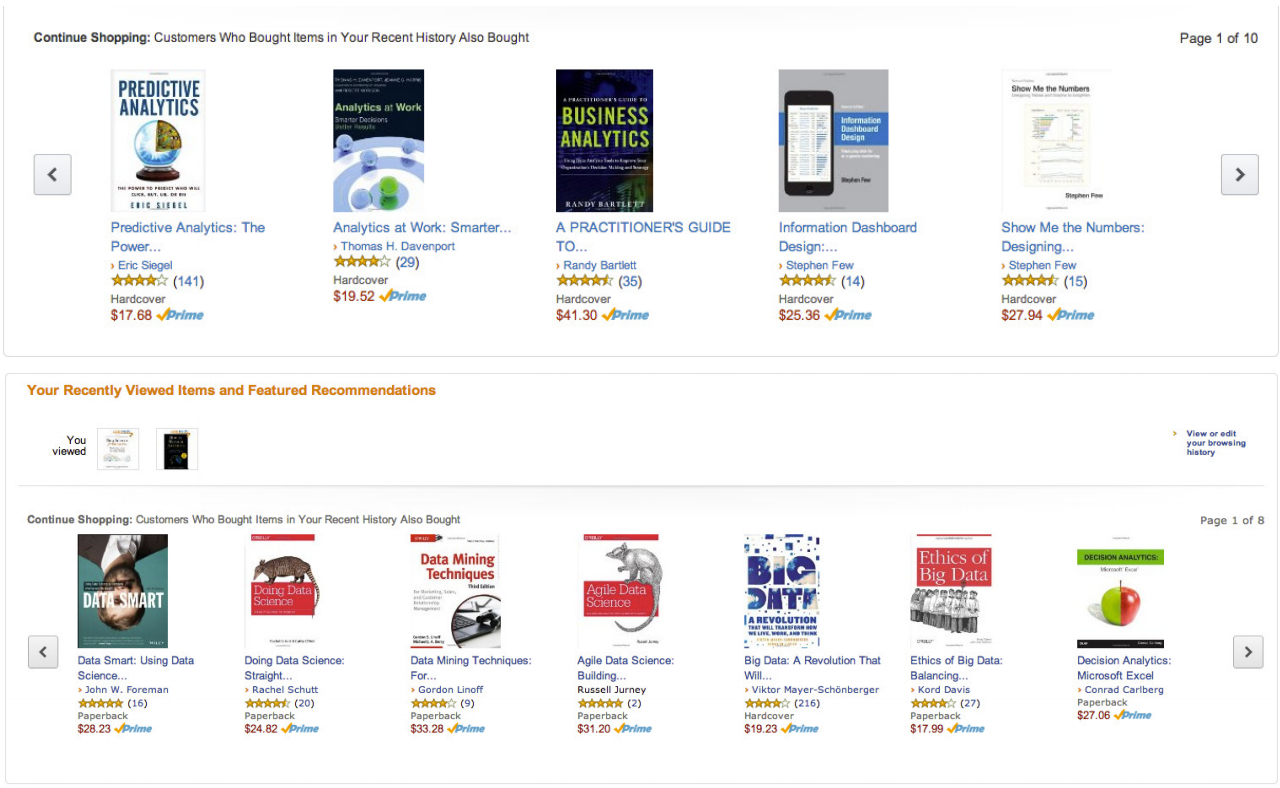
\includegraphics[width=\linewidth]{rec_list.png}
    \caption{{\se Amazon.com} 中使用者之根據購買紀錄進行推薦之商品清單(上方),以及根據使用者目前之瀏覽紀錄進行推薦之商品清單(下方)}
    \label{fig:rec_list}
    \end{center}
\end{figure}

\section{根據使用者之性格特質給予特定廣告之策略}
{Facebook 是目前最受歡迎的社群平台之一,同時大部分的使用者在 Facebook 上留下了許多個人資訊,本段對於個人資訊之定義為使用者對於何種文章類型(體育、音樂、書籍、餐廳等)表示喜歡(Like)。藉由分析使用者之個人資訊,預測使用者之年齡、性別、職業甚至是個性~\cite{kosinski2013private},進而根據不同個性之使用者投放特定廣告~\cite{matz2017psychological},是目前 Facebook 在選擇投放廣告對象之依據方法之一。此應用為透過使用者在 “ 特定網頁平台內 ” 對何種文章表示喜歡來進行大五性格特質分數的預測,而本篇論文則是透過 “ 跨網頁 ” 的瀏覽紀錄預測使用者的個人資訊以及大六性格特質分數。\par

 
針對不同性格特質給予廣告之實際影響甚至可以追朔至 $2016$ 年美國總統選舉,根據媒體報導劍橋分析公司(Cambridge Analytica)透過社群平台 Facebook 取得了 $5,000$ 萬名使用者之個人資訊~\cite{cadwalladr2018revealed}進行使用者性格特質之預測,再針對不同性格特質之使用者投放競選廣告而影響選情。縱使報導的真實性尚未確定,但是對特定性格之使用者投放特定廣告之影響力已經被證實~\cite{cadwalladr2018revealed}。

}

\section{預測使用者在特殊節日之網頁瀏覽行為變化}
{
基於我先前之研究~\cite{lien2017taai},透過與本論文相同的資料集,分析使用者在特殊節日期間與平時對於電子商務平台相關網頁瀏覽比例之比較,以使用者瀏覽網頁的種類以及使用者之性別、年齡、感情狀態當作特徵,藉由基本的監督式學習模型(K-nearest neighbors, Support vector machine, Random forest and Logistic regression) 預測使用者在特殊節日是否會提高瀏覽電子商務平台網頁之比例,例如:中秋節、單身節以及聖誕節,其預測結果如表~\ref{tab:classifier-auc}。\par

\begin{table}[tbh]
\centering
\caption{四種分類器預測結果之 AUCs 比較}
\label{tab:classifier-auc}
\begin{tabular}{c|c|c|c|c|c|c}
\hline
    & \multicolumn{2}{c|}{Moon Festival} & \multicolumn{2}{c|}{Singles Day} & \multicolumn{2}{c}{Christmas} \\ \hline\hline
    & Training & Test & Training & Test & Training & Test \\ \hline
KNN & 0.71     & 0.55 & 0.75     & 0.63 & 0.78     & 0.72 \\ \hline
LR  & 0.73     & \textbf{0.65} & 0.70     & 0.61 & 0.82     & 0.73 \\ \hline
SVM & 0.74     & 0.64 & 0.84     & \textbf{0.64} & 0.84     & \textbf{0.77} \\ \hline
RF  & 0.99     & 0.60 & 0.99     & 0.60 & 0.99     & 0.68 \\ \hline
\end{tabular}
\end{table}


基於此研究結果,我認為此研究透過使用者之網頁瀏覽歷史紀錄之應用能夠幫助電子商務平台針對不同瀏覽習慣之使用者給予特定的市場行銷手段,能夠節省廣告成本並使廣告效果最大化。
}
               % 第二章    (自行寫入)
\chapter{資料集介紹與特徵設計}
{本章總共分成三個部分,首先第一節將介紹原始資料(raw data)之詳細組成資訊,原始資料包含:網頁瀏覽歷史紀錄、使用者之詳細個人資訊以及大六性格特質測驗分數。第二節介紹資料前處理之過程與想法。第三節則說明特徵選擇之原因。}

\section{資料集中各類資訊介紹}
\subsection{資料集中網頁瀏覽歷史紀錄之介紹}
{
本篇論文所使用之資料集是取自 $672$ 位使用者之 Google Chrome 網頁瀏覽器之網頁瀏覽歷史紀錄(browsing history),大部分的網頁瀏覽歷史紀錄之紀錄期間為 $2016$ 年 $8$ 月至 $2016 $ 年 $12$ 月。所有使用者之瀏覽量為 $12,837,216$ 筆,圖~\ref{fig:webcate_distribution} 與表~\ref{tab:url-stat-summary} 分別說明每一位使用者瀏覽網頁數量之經驗分布函數與綜合統計表格。

\begin{figure}
    \graphicspath{{fig/}}
    \begin{center}
    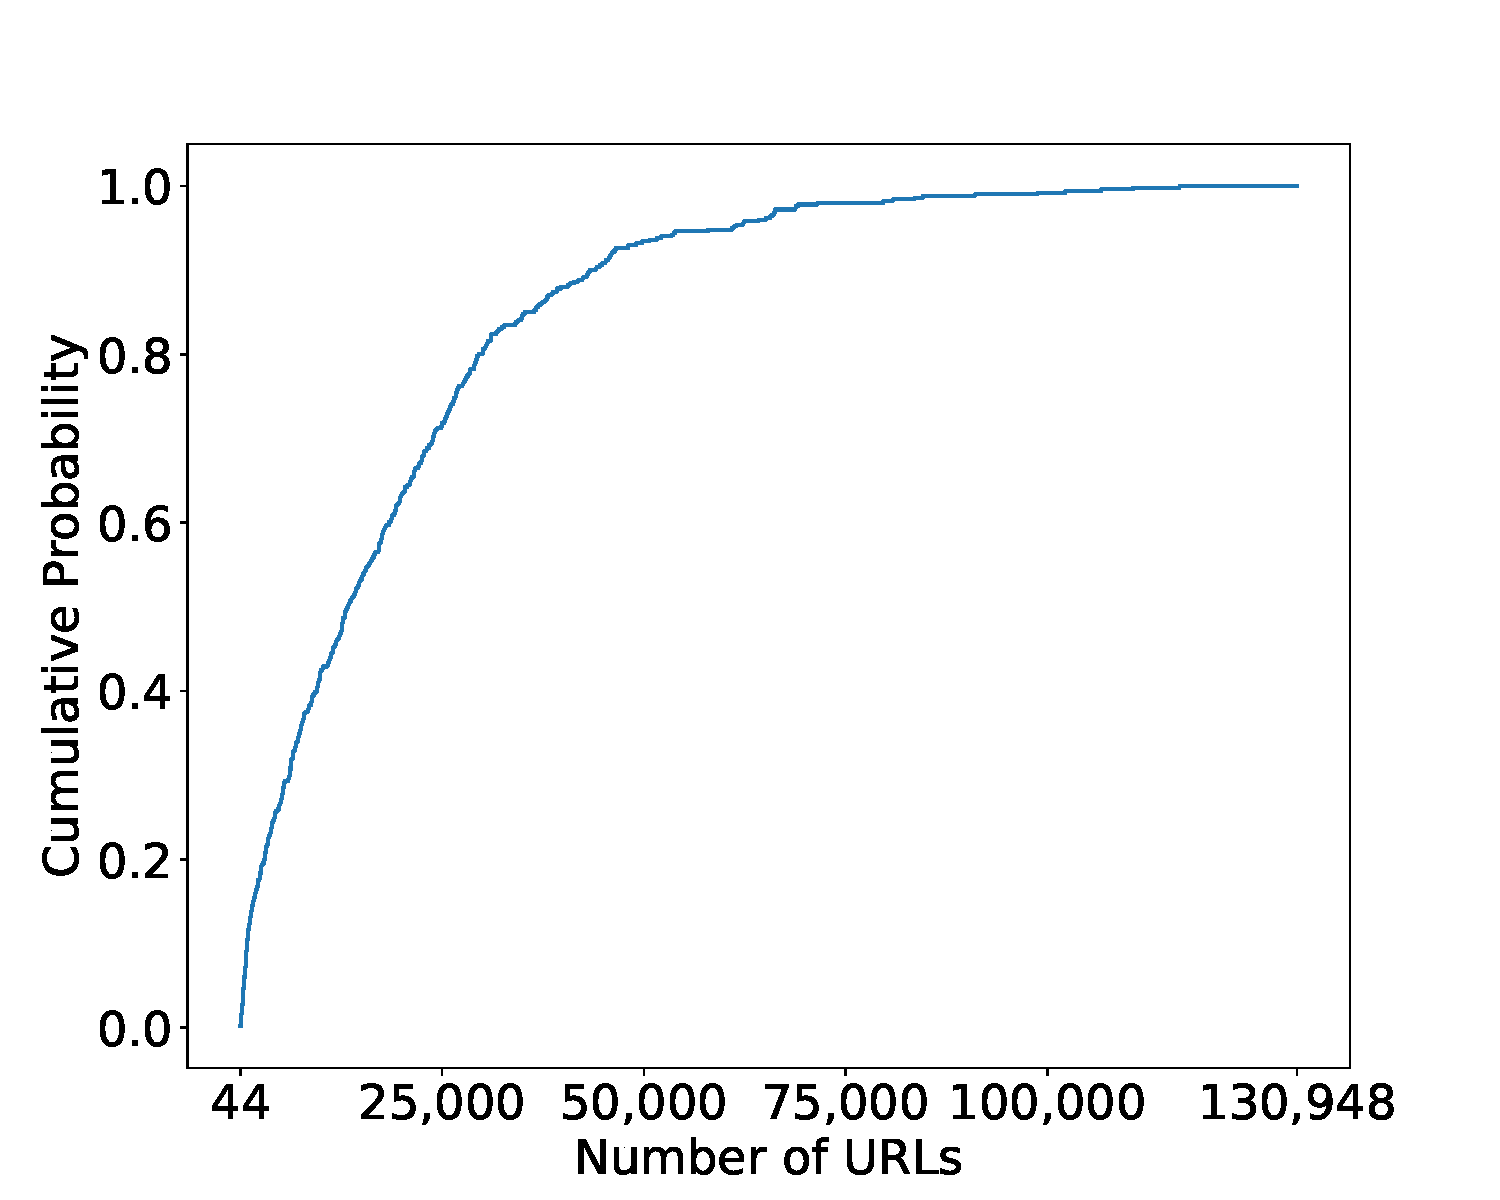
\includegraphics[scale=0.25]{summary_of_url-eps-converted-to.pdf}
    \caption{使用者瀏覽網頁數量之經驗分布函數}
    \label{fig:webcate_distribution}
    \end{center}
\end{figure}

\begin{table}[tbh]
    \centering 
    \caption{使用者瀏覽網頁數量之綜合統計} 
    \label{tab:url-stat-summary}
    \begin{tabular}{c|c|c|c|c|c} 
    \hline min & 1st Quartile & Median &Mean & 3rd Quartile & max \\
    \hline\hline $44$ & $4,239$ & $13,335$ & $19,103$ & $26,698$ & $130,992$ \\
    \hline
    \end{tabular} 
\end{table}

}
\subsection{資料集中使用者個人資訊之介紹}
{
全部具有網頁瀏覽紀錄的使用者之中共有 $508$ 位使用者具有較詳細的個人資訊(demographic information),個人資訊包含:性別、年齡以及感情狀態(單身、交往中、已婚以及其他),圖~\ref{fig:dataset_distribution} 以圓餅圖說明個人資訊之分布狀態。

\begin{figure}[h]
    \graphicspath{{fig/}}
    \begin{center}
    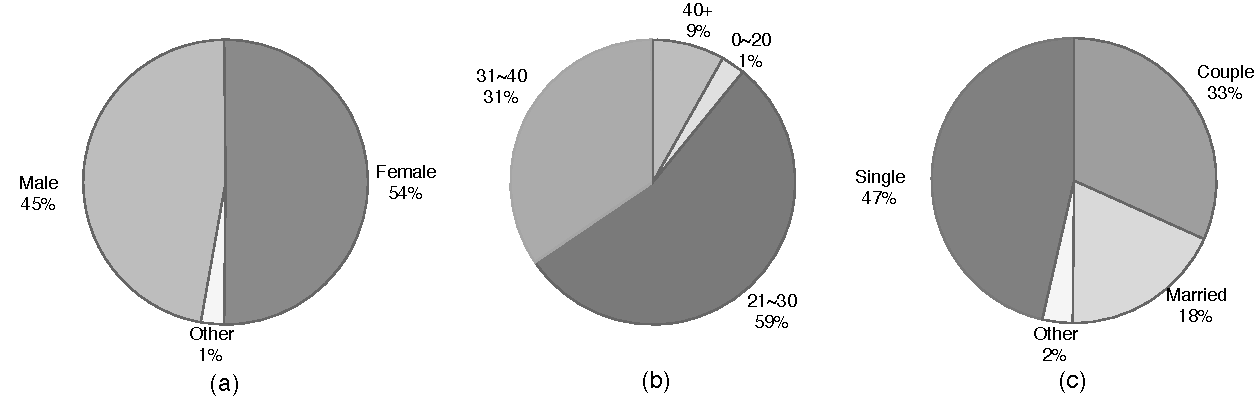
\includegraphics[scale=0.65]{fig/demo_pie.pdf}
    \caption{個人資訊分布狀態之圓餅圖,(a)性別(b)年齡(c)感情狀態}
    \label{fig:dataset_distribution}
    \end{center}
\end{figure}

}

\subsection{資料集中使用者大六性格特質之介紹}
{
全部具有網頁瀏覽紀錄之使用者中共有 $513$ 位使用者具大六性格特質測驗分數(big-six personality),其中大六性格特質包含:真誠性(Honesty-Humility)、情緒不穩定性(Neuroticism)、外向性(Extraversion)、親和性(Agreeableness)、盡責性(Conscientiousness)以及經驗開放性(Openness to Experience),各項分數分布狀態如圖~\ref{fig:pr_distribution}。大六性格特質為大五性格特質的延伸,大六性格特質增加了真誠性(Honesty-Humility)作為構成人的主要性格特徵,而大五性格特質在現代心理學中已經被認為是代表所有人格特質中的基本架構~\cite{o2002quantitative}。 \par

\begin{figure}[h]
    \graphicspath{{fig/}}
    \begin{center}
    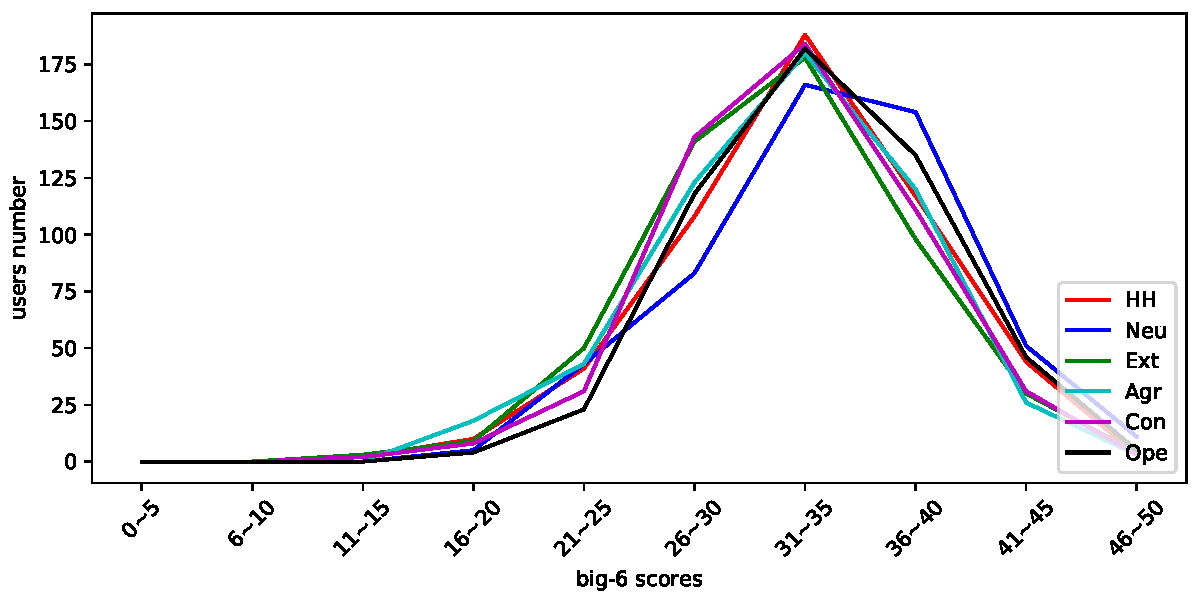
\includegraphics[scale=0.6]{fig/pr_dist.pdf}
    \caption{使用者之大六性格特質測驗分數分布狀態}
    \label{fig:pr_distribution}
    \end{center}
\end{figure}


使用者擁有三種資料集(使用者網頁瀏覽紀錄、使用者詳細個人資訊以及使用者之大六性格測驗分數)之間的人數集合關係可以透過圖~\ref{fig:dataset_distribution} 來了解,使用者具有網頁瀏覽紀錄人數為 $672$ 人,使用者具有詳細個人資訊之人數為 $508$ 人,使用者具有大六性格特質測驗分數為 $513$ 人,其中具有個人資訊之使用者皆具有大六性格特質測驗分數以及網頁瀏覽紀錄,而擁有大六性格特質測驗分數的使用者同時也擁有網頁瀏覽紀錄。

\begin{figure}[h]
    \graphicspath{{fig/}}
    \begin{center}
    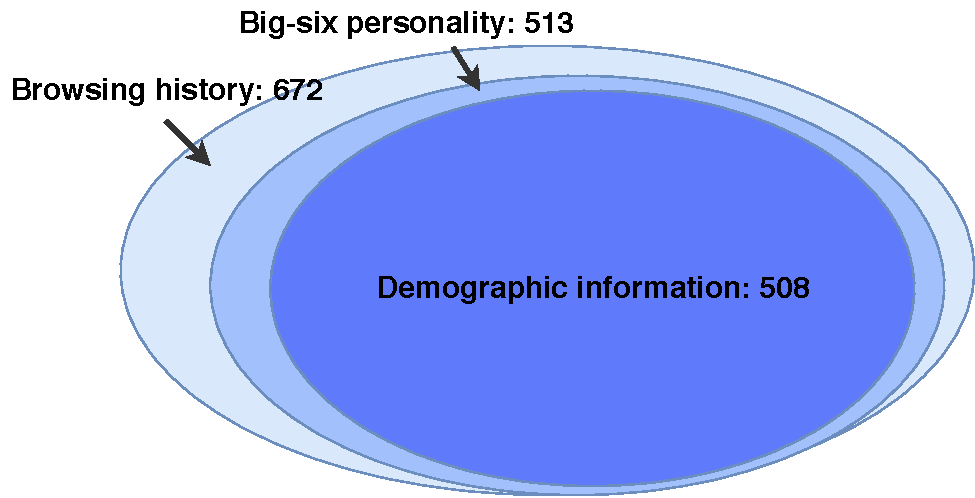
\includegraphics[scale=0.7]{fig/dataset_distribution.pdf}
    \caption{使用者中擁有三種資料集之間的人數集合關係}
    \label{fig:dataset_distribution}
    \end{center}
\end{figure}
}



\section{資料前處理之過程與想法}
{
原始資料集中分為三個部分,使用者之網頁瀏覽紀錄、使用者之個人資訊以及大六性格特質測驗分數,我將整體實驗架構訂為利用使用者之網頁瀏覽紀錄來預測使用者之個人資訊以及大六性格特質測驗分數。首先,我必須從使用者之網頁瀏覽紀錄找出特徵,起初我直接以使用者網頁瀏覽紀錄中的網址( URL)當作特徵,但是太多較為冷門的網頁只有極少部分的使用者瀏覽過,而熱門網頁所佔比例過高,例如:全部的使用者網頁瀏覽紀錄中最熱門之網頁為  facebook.com,佔全部網頁瀏覽紀錄的 $27.6\%$,圖~\ref{fig:url_popul} 為網頁瀏覽紀錄中的網址根據使用者瀏覽次數當作熱門程度之排名與使用者點擊次數之比較圖。基於此現象將造成特徵過於不平衡,所以我認為必須將特徵設定成網頁之種類較為合適。\par


因此資料前處理之第一步為將網頁瀏覽歷史紀錄中的網址(URL)透過網頁分類器進行分類\footnote{\url{http://www.fortiguard.com/webfilter}},網頁分類器能透過輸入網址後輸出對應的網頁類型,例如:輸入網址為 https://www.google.com/,則輸出之網頁類型為 “ Search Engines and Portals ”,以及輸入網址為 https://www.facebook.com/,則輸出之網頁類型為 “ Social Networking services ”。將所有使用者網頁瀏覽紀錄之網址進行分類後,總共包含88種網頁類型,進行統計後發現最熱門的網頁類型為 “ Social Networking services(SNS) ” 其次為 “ Search Engines and Portals ”,圖~\ref{fig:cate_pie} 為網頁類型佔所有瀏覽紀錄中之前五名之圓餅圖。\par

由於所有使用者網頁瀏覽歷史記錄的網址中最多瀏覽次數的網址前四名分別為 “ https://www.facebook.com/ ”、 “ https://www.google.com.tw/ ”、“ https:// mail.google.com/ ” 以及 “ https://www.youtube.com/ ”,分別佔全部的網頁瀏覽記錄中的 $27.6\%$、$11.8\%$、$6.6\%$ 以及 $6.4\%$,相對於其他網頁類型種類是相對高的,我最後再將這四種網址從網頁類別獨立出來當作 4 種獨立的網頁類型,因此網頁種類為 92 種。
}


\begin{figure}[h]
    \graphicspath{{fig/}}
    \begin{center}
    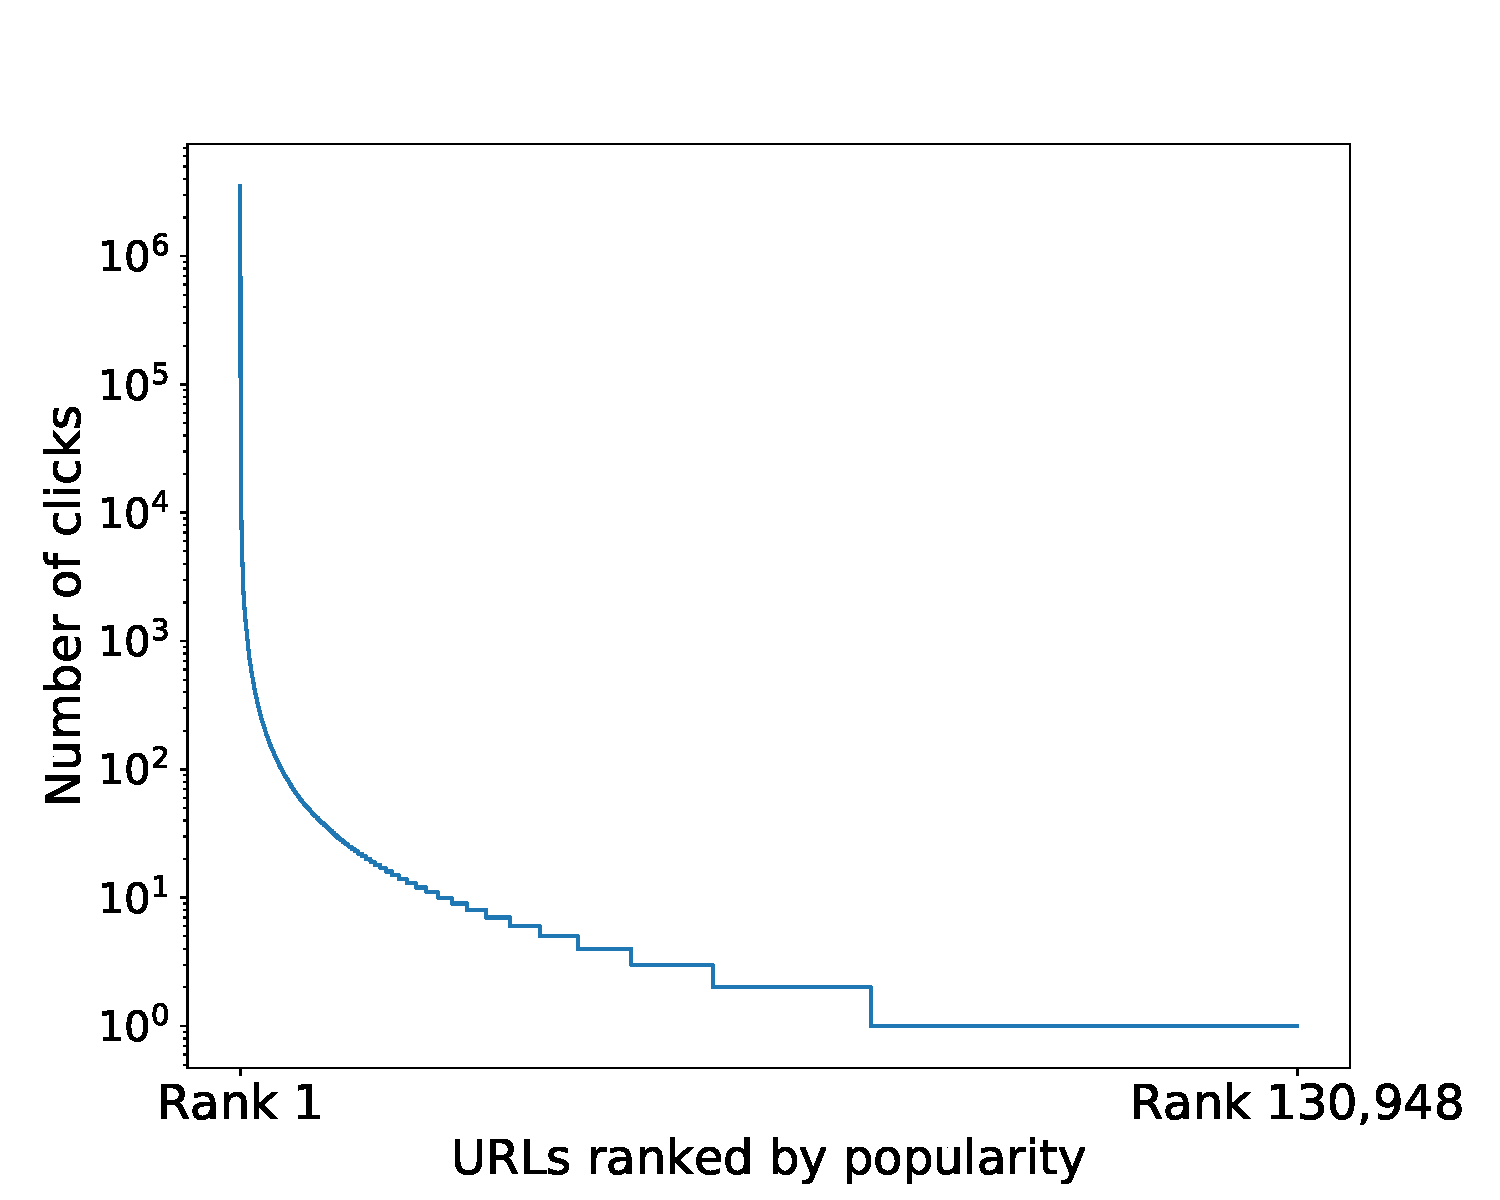
\includegraphics[scale=0.35]{fig/Proportion_of_url-eps-converted-to.pdf}
    \caption{使用者點擊次數與 URLs 熱門度排名之關係}
    \label{fig:url_popul}
    \end{center}
\end{figure}

\begin{figure}[h]
    \graphicspath{{fig/}}
    \begin{center}
    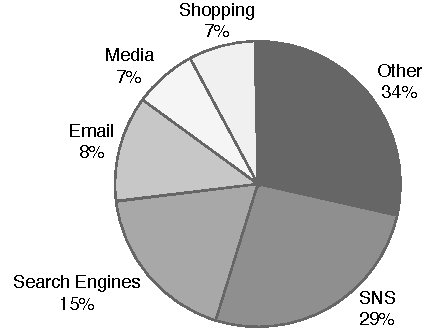
\includegraphics[scale=0.8]{fig/cate_pie.pdf}
    \caption{使用者網頁瀏覽紀錄之前五熱門類型種類比例}
    \label{fig:cate_pie}
    \end{center}
\end{figure}

\section{特徵選擇之原因以及分析}
{
呈 3.2 所說明將原始網頁瀏覽紀錄之網址轉化為網頁類型後,我將分為兩部分生成特徵,第一部分以使用者網頁瀏覽之類型作為依據,找出使用者之網頁瀏覽紀錄各類型網頁所佔之比例當作特徵,第二部分則是以使用者一天中在哪些時段瀏覽網頁之比例當作特徵。
}


\subsection{使用者於各類型網頁之瀏覽比例}
{
使用者之間的關聯性與瀏覽之網頁類型具有較高的關聯性,例如:年輕男性學生族群對於遊戲類型的網頁具有較高的瀏覽率,而銀行金融類型之網頁類型則對於年紀相對高的族群有較高的吸引力。因此以每一位使用者在各類型網頁的瀏覽比例當作特徵進行分析我認為是合適的選擇,而計算每一位使用者之在各類型網頁的瀏覽比例之算法為式(3.1),將使用者瀏覽過第 $i$ 種網頁類型之次數除以使用者之總瀏覽次數,作為使用者瀏覽第 $i$ 種網頁類型之比例,$cate_i$ $ratio$ 中 $i$ 為 $0\sim91$,分別代表 92 種不同的網頁類型。


    $$cate_i\mbox{ }ratio=\frac{\mbox{number of visits on the }cate_i\mbox{ websites}}{\mbox{total number of visits}} \eqno {(3.1)}$$

}

\section{使用者於一天中各時段之瀏覽頻率}
{
每一位使用者都有特定生活作息,我認為擁有類似生活作息的使用者之間可能擁有較高的關聯性,例如:大學生族群比較傾向晚睡,因此其在凌晨時段相對於其他使用者擁有較高的瀏覽比例。藉由使用者一天 24 個時段之中在各時段之瀏覽紀錄來統計每一位使用者在哪些時段瀏覽頻率較高,便能夠區分出各使用者族群。\par


其中定義使用者在同一天內擁有超過 30 筆瀏覽紀錄才能夠被認定當天有確切的瀏覽行為發生,並且在同一個時段內擁有超過 10 筆瀏覽紀錄才能夠被認定該時段確實有進行網頁瀏覽。而詳細的計算方式為式(3.2),使用者第 $i$ 個時段之網頁瀏覽頻率為使用者之網頁瀏覽紀錄中第 $i$ 個時段發生網頁瀏覽行為天數除以使用者有瀏覽行為天數總和,$timesession_i$ $ratio$中 $i$ 為 $0\sim23$,分別代表 0 時至 23 時之時段。

    $$timesession_i\mbox{ }ratio=\frac{\mbox{number of days have browsing behaviors in }timesession_i}{\mbox{number of days have browsing behaviors}} \eqno {(3.2)}$$
}


               % 第二章    (自行寫入)
\chapter{預測使用者個人資訊與大六性格特質分數之方法}
{
首先定義預測使用者個人資訊與大六性格特質分數分別為分類問題以及回歸問題。對於使用者個人資訊之預測,先將 3 種個人資訊進行分類(1)性別分為:男性、女性以及其他,共 3 類、(2)年齡分為:$16\sim20$、$21\sim25$、$26\sim30$、$31\sim35$、$36\sim40$、$41\sim45$ 以及 $46$ 以上,共 7 類、(3)感情狀態分為:單身、交往中、已婚、其他以及不公開,共 5 類。而大六性格特質分數則是介於 0 至 50 分,分別為真誠性({\se Honesty-Humility})、情緒不穩定性({\se Neuroticism})、外向性({\se Extraversion})、親和性({\se Agreeableness})、盡責性({\se Conscientiousness})以及經驗開放性({\se Openness to Experience})。\par
於此章中,將會以兩種方法預測使用者個人資訊與大六性格特質分數,分別為基於監督式學習之預測,以及透過將使用者分群後再以監督式學習進行預測,並分別介紹其中所使用之分類器以及分群方法。

}


\section{預測個人資訊之分類模型選擇}
{
由於預測個人資訊屬於分類問題,因此選用 k-Nearest Neighbor(k-NN)~\cite{altman1992introduction}、\\
Random forests ~\cite{ho1995random}、Logistic regression 以及 Support vector machine(SVM) 作為分類器進行個人資訊之預測。其中 k-NN 主要透過參考以使用者之特徵當作座標,找出當前使用者與其他使用者之中最接近之 k 位使用者當作預測依據。Random forests 則是以使用者之特徵當作分支條件透過 decision tree 的方式找出使用者之種類。Logistic regression 則是透過給予所有使用者特徵權重相加,與 Linear regression 方法類似,差別在於 Logistic regression 透過激勵函數(activation function)將輸出值壓縮至 0 到 1 之間成為判斷類別之機率。SVM 為 Hinge loss(式 4.1,$y$ 為預測值、$t$ 為實際值)加上透過 Kernel method 解決特徵向量投影到高維度平面後計算負擔過大的問題之方法。 

$$L(y)=\max (0, 1-t\cdot y) \eqno {(4.1)}$$

}
\section{預測大六性格特質分數之回歸模型選擇}
{
由於大六性格特質分數屬於數值回歸問題,我嘗試了 Linear regression 以及 SVM。其中基於 Linear regression 我將介紹 Lasso regression、 Ridge regression 以及 Elastic net regression,並在第五章進行不同模型之預測結果比較。首先,Lasso regression ~\cite{tibshirani1996regression}為線性最小平方法(linear least squares function)作為 loss function,並經過 L1-norm regularization 之方法,其目標函數定義為下列式 4.2,其主要優勢在於以 L1-norm regularization 所找到最佳解之變數係數經常為 0,因此能夠解決變數選擇問題。\par

    $$\beta=\arg \min_\beta \left[ \frac{1}{2}\sum_{i=1}^n(\hat{y_i} - y_i)^2+\lambda \parallel \beta \parallel_1\right]\eqno {(4.2)}$$

Ridge regression ~\cite{hoerl1970ridge}同樣以線性最小平方法(linear least squares function)作為 loss function,但與 Lasso regression 不同之處在於 Ridge regression 是 L2-norm regularization,因此 Ridge regression 之目標函數可定義成下列式 4.3。\par

    $$\beta=\arg \min_\beta \left[ \frac{1}{2}\sum_{i=1}^n(\hat{y_i} - y_i)^2+\lambda \parallel \beta \parallel_2\right]\eqno {(4.3)}$$
 
而 Elastic net regression 則是綜合了 Lasso regression 與 Ridge regression,同時具有  L1-norm 與  L2-norm regularization,因此 Elastic net regression 之目標函數可定義成下列式 4.4。

    $$\beta=\arg \min_\beta \left[ \frac{1}{2}\sum_{i=1}^n(\hat{y_i} - y_i)^2+\lambda_1 \parallel \beta \parallel_1+\lambda_2 \parallel \beta \parallel_2\right]\eqno {(4.3)}$$

\clearpage
}

\section{結合分群方法之監督式學習}
{
基於相似網頁瀏覽習慣之使用者可能具有類似的特徵分布,因此我猜想若將使用者分群後,將類似的使用者以監督式學習進行個人資訊與大六性格分數預測,相對於直接以全部的使用者特徵進行預測是能夠提高預測結果之準確性。\par

將使用者依據其特徵利用 $k$ - 平均演算法(k-means clustering)進行分群,其目標函數定義為式 4.4,其中 $(x_1,x_2,…,x_n)$ 代表 $n$ 位使用者之特徵向量,將 $n$ 位使用者歸類成 $k$ 個類別 $S=(S_1,S_2,…,S_k)$,$\mu_i$ 為 $S_i$ 中所有使用者的特徵向量平均值,並使其盡量滿足每個類別中平方和(within-cluster sum of squares)為最小值。\par

    $$S=\arg \min_S \sum_{i=1}^k \sum_{x\in S_i} \parallel x-\mu_i\parallel^2 \eqno {(4.4)}$$
    
透過 k-means 將使用者分群之後,再藉由 4.1、4.2 所介紹之方法對每一群使用者進行訓練,並預測其個人資訊以及大六性格特質分數。
\clearpage
}
\chapter{實驗結果與分析}
{
本章節將介紹第三章提到的資料集於本實驗中 training data 與 test data 之分配方式,以及介紹評估實驗結果之方法。最後比較基於監督式學習與透過對使用者分群之後再以監督式學習之預測結果,並對實驗結果提出結論與分析。
}

\section{實驗資料集介紹}
{
基於第三章所介紹的資料集,本實驗透過交叉驗證(5-fold cross validation)的方式,將資料集依據使用者分割成 5 份子樣本,將其中 1 份單獨的子樣本當作驗證模型的資料,而其他 4 份子樣本用來訓練模型,重複 5 次,將每一份子樣本都進行驗證 1 次,最後將 5 次驗證結果取平均,最後得到 1 個能夠評估此模型的單一值。


}

\section{評估模型優劣之方法}
{
由於使用者個人資訊之預測屬於多類別(multi-class)之分類問題,而使用者大六性格特質分數之預測屬於數值回歸問題,兩者所使用的評估標準不相同,因此本節將針對兩種不同問題的預測模型分別進行評估方法之介紹。


}
\subsection{個人資訊預測結果之評估標準}
{
基於分類問題,大部分以 $F_1$ score 進行準確度評估,$F_1$ score 主要在召回率(recall)與精確率(precision)之間取得平衡,透過圖~\ref{fig:dtt} 中定義的 TP、FP、FN、TN 來進行召回率、精確率以及 $F_1$ score 之計算,其公式如下。\par

$$F_1 \mbox{ } score = 2 \cdot \frac{precision \cdot recall}{precision + recall} \eqno{(5.1)}$$

$$Precision = \frac{tp}{tp+fp} \eqno{(5.2)}$$

$$Recall = \frac{tp}{tp+fn} \eqno{(5.3)}$$

\begin{figure}[h]
    \graphicspath{{fig/}}
    \begin{center}
    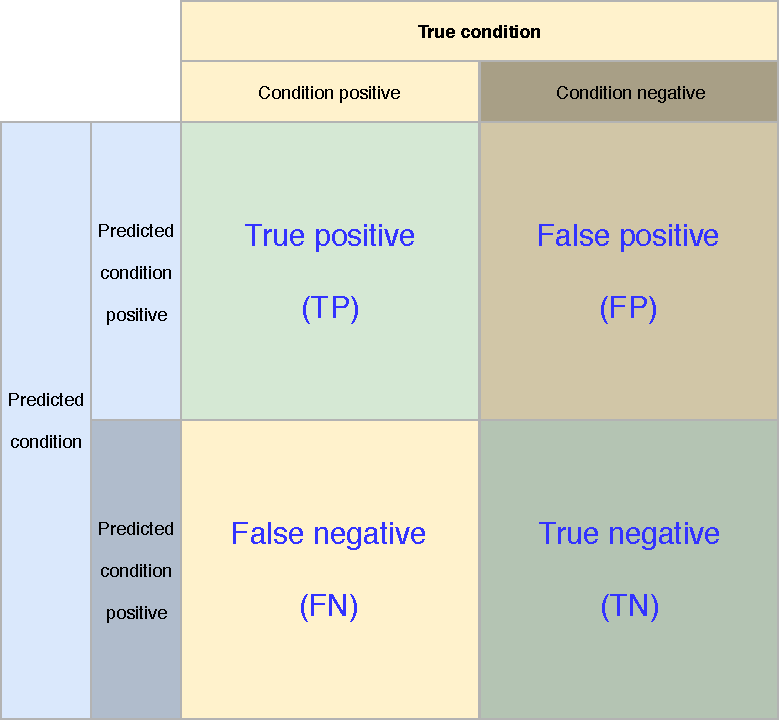
\includegraphics[scale=0.7]{fig/dtt.pdf}
    \caption{diagnostic testing table}
    \label{fig:dtt}
    \end{center}
\end{figure}


而本實驗中預測使用者之個人資訊為 multi-class 分類方法,因此無法直接使用 $F_1$ score 當作評估標準,必須改以 $MicroF_1$ 與 $MacroF_1$ 對 multi-class 分類進行評估,其公式如式 5.4、5.5, $MicroF_1$ 將 TP、FP、FN、TN 各進行累加後再計算其 $F_1$ score,而 $MacroF_1$ 則是將每一種類別之 $F_1$ score 計算出來後再取平均。其中 $MicroF_1$ 與 $MacroF_1$ 最明顯的差異在於,$MicroF_1$ 較不考慮每一種類別之間的樣本數量的平衡狀況,而在 $MacroF_1$ 的計算方式下,樣本數較少的類別對於整體分數的影響等同於其他類別,因此再選擇評估標準時,必須考慮資料集中樣本類別間是否平均,而本實驗所使用之資料集,每一種類別之樣本數較為不平衡,因此選擇以 $MicroF_1$ 作為評估標準。

$$MicroF_1=\frac{2\cdot \sum_{i=1}^C{TP_i}}{2\cdot \sum_{i=1}^C{TP_i} + \sum_{i=1}^C{FP_i} + \sum_{i=1}^C{FN_i}} \eqno {(5.4)}$$

$$MacroF_1 = \frac{1}{C} \sum_{i=1}^C{\frac{2\cdot TP_i}{2\cdot TP_i+FP_i+FN_i}} \eqno {(5.5)}$$




}

\subsection{大六性格特質分數預測結果之評估標準}
{
對於數值預測結果之評估標準,本篇論文以均方根誤差(root-mean-square error)進行評估,$RMSE$ 為一種經常用來測量數值之間差異性的量度,其計算方式如式 5.6,其中 $\hat{y}$ ̂為樣本實際值、$y$ 為預測值、$n$ 為預測樣本總數。

$$RMSE = \sqrt{\frac{ \sum_{t=1}^n{(y_t-\hat{y_t})^2 }}{n}} \eqno{(5.6)}$$

}

\subsection{使用者分群效果之評估標準}
{
第四章中介紹藉由 k-means 將使用者進行分群,本篇論文選擇 Silhouette score~\cite{de2015recovering}作為分群效果之評估標準。式 5.7 中 $s(i)$ 為第 i 位使用者之 Silhouette score,$a(i)$ 為第 i 位使用者與同群之其他使用者之間的平均距離,$b(i)$ 為使用者 $i$ 與不同群之其他使用者間的最小平均距離。而式 5.7 等價於式 5.8 因此可以了解當 $s(i)=0$ 時表示第 $i$ 位使用者剛好介於兩群之交界處,若 $s(i)<0$ 則表示第 $i$ 位使用者介於兩群之重疊處,因此當 Silhouette score $<0$ 則表示分群效果不佳。

$$s(i)= \frac{b(i)-a(i)}{\max (a(i),b(i))} \eqno{(5.7)}$$

\begin{equation}
\setcounter{equation}{8}
s(i)=
\left\{
     \begin{array}{lr}
     1-\frac{a(i)}{b(i)}, & \mbox{if }a(i)<b(i)\\  
     0, & \mbox{if }a(i)=b(i)\\  
     \frac{b(i)}{a(i)}-1, & \mbox{if }a(i)>b(i)    
     \end{array}
\right .
\end{equation}
}

\section{預測個人資訊之結果比較}
{
本節將介紹 4 種分類器:k-NN、Random forests、Logistic regression 以及 SVM 之參數設定,並在最後透過混淆矩陣(confusion matrix)以及 $MicroF_1$ 之分數比較 “基於監督式學習” 與 “結合分群之監督式學習” 兩者年齡、性別、感情狀態之預測結果。 \par

\clearpage

基於監督式學習之預測方法中,當使用 k-NN 作為分類器時,先利用 $MicroF_1$ 找出最佳k之值,並以此值產生混淆矩陣評估整體預測結果。如圖~\ref{fig:super_knn_microf1},呈現 k-NN 中當 $k$ 之值從 1 增加至 20 其預測年齡、性別、感情狀態之 $MicroF_1$ 分數,其最大值分別為 $k=18$、$k=19$、$k=5$,$MicroF_1$ 分別為 $0.427$、$0.594$、$0.478$,再將 3 種不同的 $k$ 值之 k-NN 預測結果以混淆矩陣呈現,如圖 ~\ref{fig:knn_con} 左側中 y 軸為 true label 值、x 軸為 predicted label,矩陣中間之值為預測樣本數與其比例,透過混淆矩陣可以清楚觀察到各種類之預測狀況。\par

\begin{figure}[h]
    \graphicspath{{fig/}}
    \begin{center}
    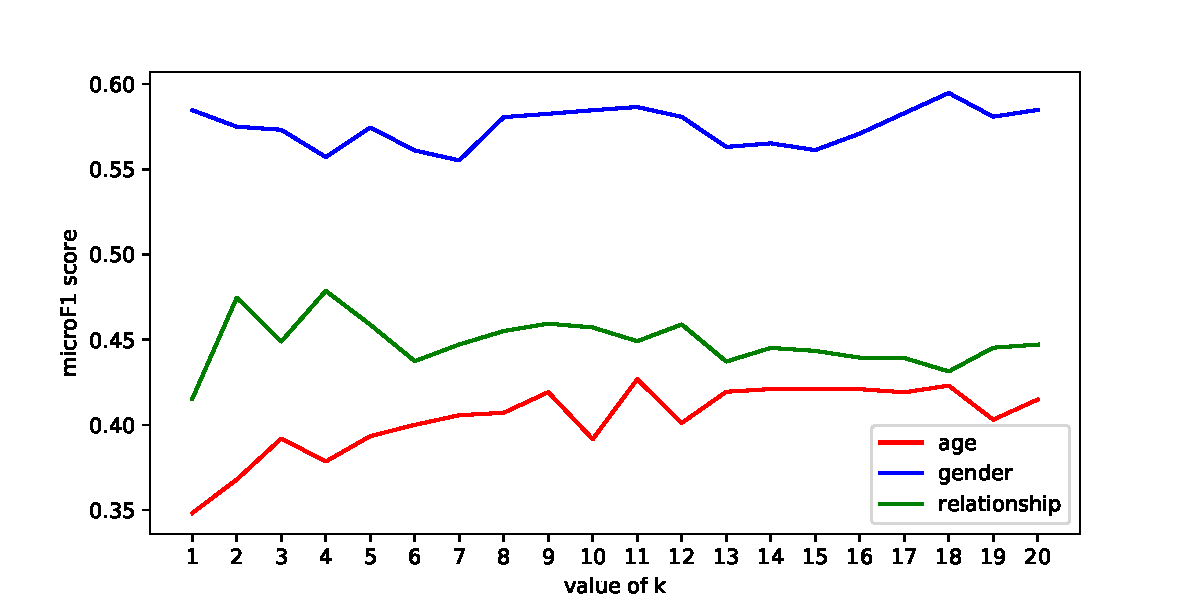
\includegraphics[scale=0.5]{fig/super_knn_microf1.pdf}
    \caption{k-NN 中根據不同 k 值對應之 $MicroF_1$ 分數}
    \label{fig:super_knn_microf1}
    \end{center}
\end{figure}


使用 Random forests 作為分類器時,由於其中決策樹之深度可以進行調整,因此同樣使用 $MicroF_1$ 進行不同最大深度($max \_depth$)之預測效果比較(圖~\ref{fig:super_rf_microf1}),其最佳年齡、性別以及感情狀態之最大深度值分別為 8、5、9,其 $MicroF_1$ 分別為 $0.453$、$0.697$、$0.488$,而最佳深度之混淆矩陣如圖~\ref{fig:rf_con} 左側。\par

\begin{figure}[h]
    \graphicspath{{fig/}}
    \begin{center}
    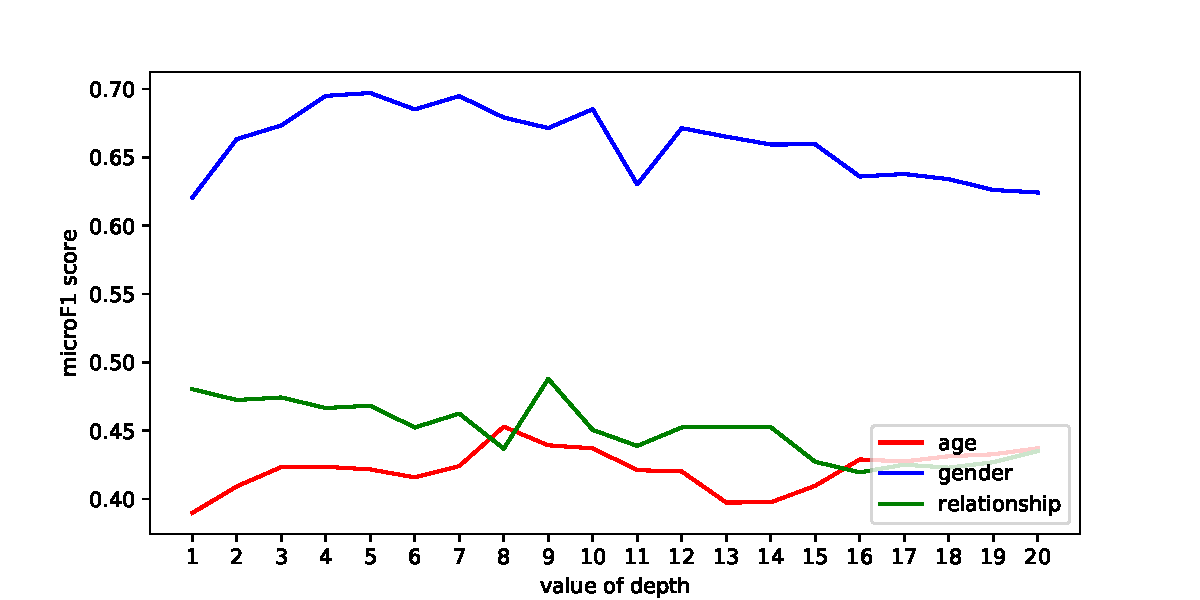
\includegraphics[scale=0.5]{fig/super_rf_microf1.pdf}
    \caption{ Random forests 中根據不同 $max \_depth$ 值對應之 $MicroF_1$ 分數}
    \label{fig:super_rf_microf1}
    \end{center}
\end{figure}
\clearpage

使用 Logistic regression 與 SVM 當作分類器時,能夠透過調整其中 regularization term 之權重($C$)找出最佳預測效果,因此同樣也利用 $MicroF_1$ 找出最佳權重分配, Logistic regression 對年齡、性別、感情狀態預測結果之 $MicroF_1$ 分別為 $0.427$、$0.697$、$0.476$,而 SVM 之預測結果 $MicroF_1$ 分別為 $0.388$、$0.591$、$0.474$,並以混淆矩陣呈現 Logistic regression 預測結果
(圖~\ref{fig:lr_con} 左側)與 SVM 預測結果(圖~\ref{fig:svm_con} 左側)。\par

結合分群之監督式學習的預測方法中,將透過 k-means 將使用者分群並以 Silhouette score 決定分群數量(圖~\ref{fig:silhouette_score} 為 Silhouette score 之分布),由於當 $k<6$ 時 Silhouette score 下降幅度較為明顯,因此本實驗決定將分群數量定為 2 到 6 群,再以 k-NN、Random forests、Logistic regression 以及 SVM 對分群後的使用者進行個人資訊之預測,最後將以 $MicroF_1$ 決定其中分類器之參數設定,並以混淆矩陣呈現預測結果。\par

\begin{figure}[h]
    \graphicspath{{fig/}}
    \begin{center}
    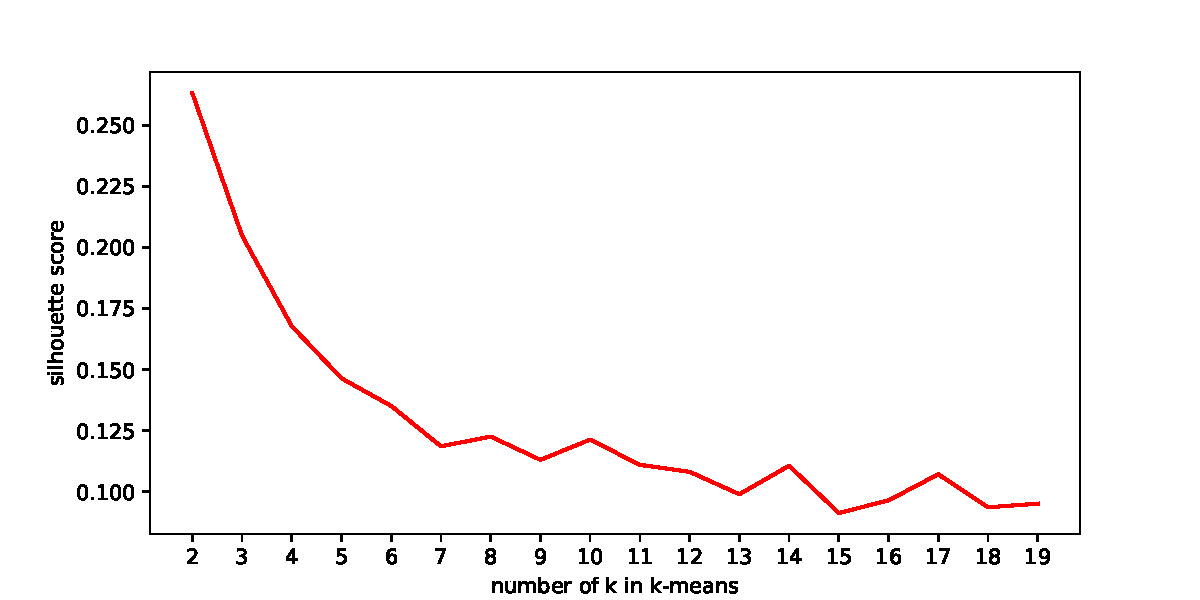
\includegraphics[scale=0.6]{fig/silhouette_score.pdf}
    \caption{分群數量之 Silhouette score 分布}
    \label{fig:silhouette_score}
    \end{center}
\end{figure}

以 k-NN 作為分類器時,年齡之最佳分群數量為 3 群、最佳 $k$ 值為 20,性別之最佳分群數量為 5 群、最佳 $k$ 值為 15,感情狀態之最佳分群數量為 3 群、最佳 $k$ 值為 3,其分群效果以混淆矩陣來表示,如圖 ~\ref{fig:knn_con} 右側。\par

以 Random forests 作為分類器時,年齡之最佳分群數量為 3 群、最佳 $max\_depth$ 值為 20,性別之最佳分群數量為 5 群、最佳 $max\_depth$ 值為 15,感情狀態之最佳分群數量為 3 群、最佳 $max\_depth$ 值為 3,其分群效果以混淆矩陣來表示,如圖~\ref{fig:rf_con} 右側。\par

以 Logistic regression 作為分類器時,年齡之最佳分群數量為 3 群、最佳 $C$ 值為 20,性別之最佳分群數量為 5 群、最佳 $C$ 值為 15,感情狀態之最佳分群數量為 3 群、最佳 $C$ 值為 3,其分群效果以混淆矩陣來表示,如圖~\ref{fig:lr_con} 右側。\par

以 SVM 作為分類器時,年齡之最佳分群數量為 5 群、最佳 $C$ 值為 20,性別之最佳分群數量為 5 群、最佳 $C$ 值為 15,感情狀態之最佳分群數量為 3 群、最佳 $C$ 值為 3,其分群效果以混淆矩陣來表示,如圖~\ref{fig:svm_con} 右側。\par

表~\ref{tab:demo_f1}呈現以 4 種分類器與總是預測使用者數量最多的類別(baseline)中利用 “基於監督式學習” 、 “結合分群監督式學習” 預測年齡、性別、感情狀態之 $MicroF_1$ 分數,透過此表格能夠清楚了解經過分群後預測個人資訊之效能大部分都有提高,對於性別之預測 “基於監督式學習” 有較好的表現,而在年齡、感情狀態之預測 “結合分群監督式學習” 預測較為準確。


\renewcommand{\arraystretch}{1.5}  
\begin{table}[h]  
  
  \centering  
  \fontsize{12}{20}\selectfont  
  \caption{基於監督式學習與結合分群監督式學習之預測 $MicroF_1$ 分數比較表}  
  \label{tab:demo_f1}  
    \begin{tabular}{|c|c|c|c|c|c|c|}  
    \hline  
    \multirow{Classifier}&  
    \multicolumn{3}{c|}{基於監督式學習}&\multicolumn{3}{c|}{結合分群監督式學習}\cr\cline{2-7}  
    &Age&Gender&Relationship&Age&Gender&Relationship\cr  
    \hline  
    \hline  
    Baseline&0.388&0.545&0.474&0.411&0.598&0.476\cr\hline  
   k-NN&0.427&0.594&0.478&0.435&0.618&0.482\cr\hline  
    Random forests&0.453&{\bf 0.697}&0.488&0.419&0.687&{\bf 0.512}\cr\hline  
    Logistic regression&0.427&{\bf 0.697}&0.476&{\bf 0.457}&0.675&0.498\cr\hline  
    SVM&0.388&0.591&0.474&0.411&0.642&{\bf 0.512}\cr\hline
    \end{tabular}  
\end{table}  


\begin{figure*}[h]
    \centering
    \begin{subfigure}
      \centering
      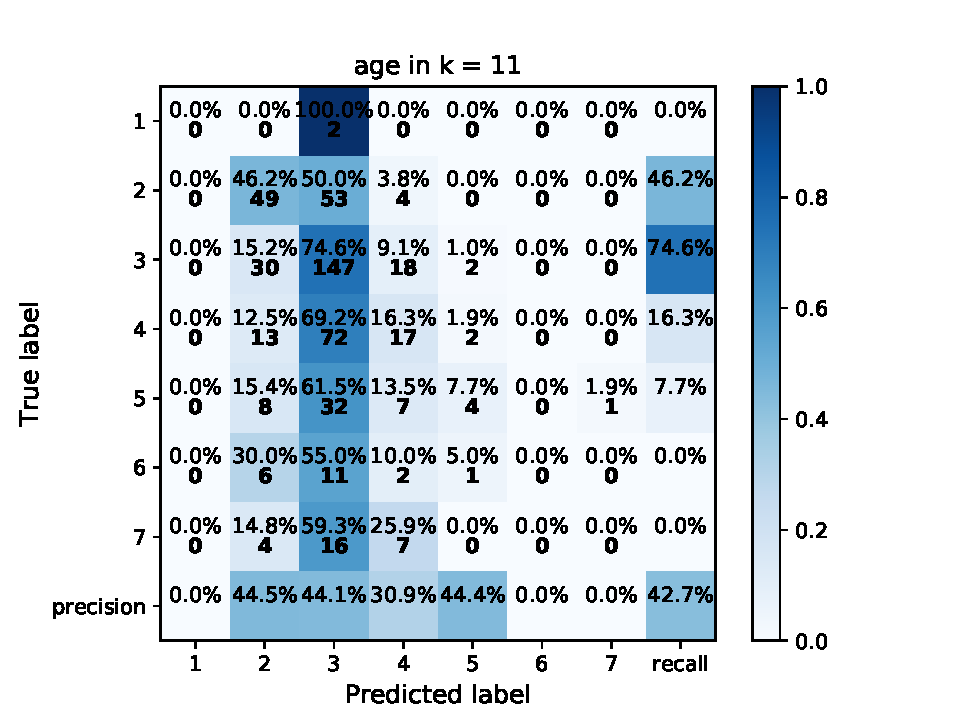
\includegraphics[scale=0.45]{fig/super_knn_age.pdf}
    \end{subfigure}%
    \begin{subfigure}
      \centering
      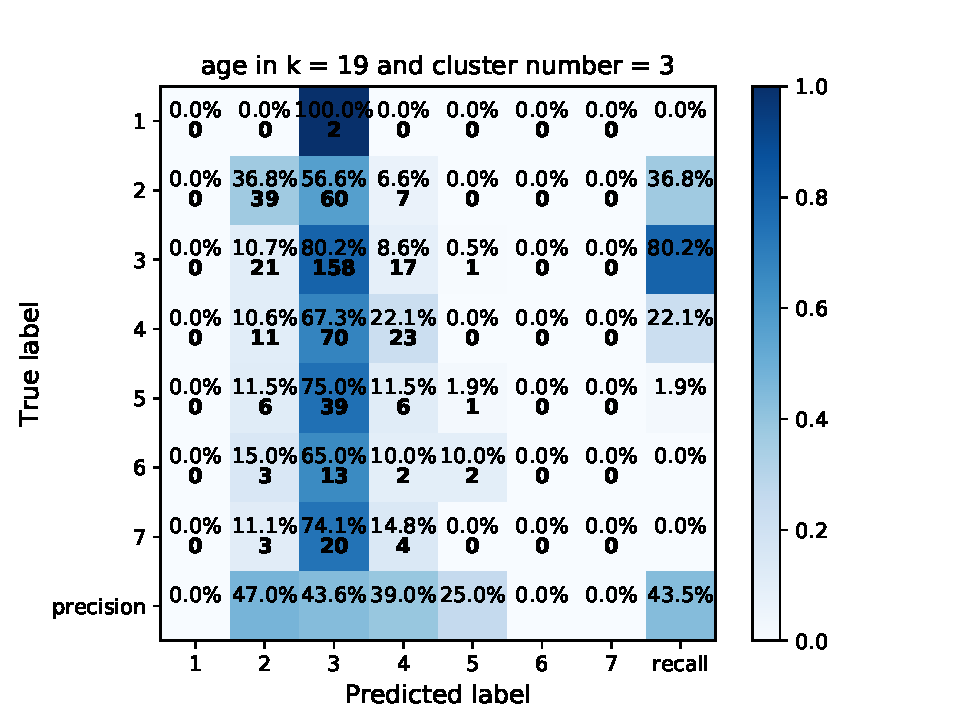
\includegraphics[scale=0.45]{fig/kms_knn_age.pdf}
    \end{subfigure}
\end{figure*}

\begin{figure*}[h]
    \centering
    \begin{subfigure}
      \centering
      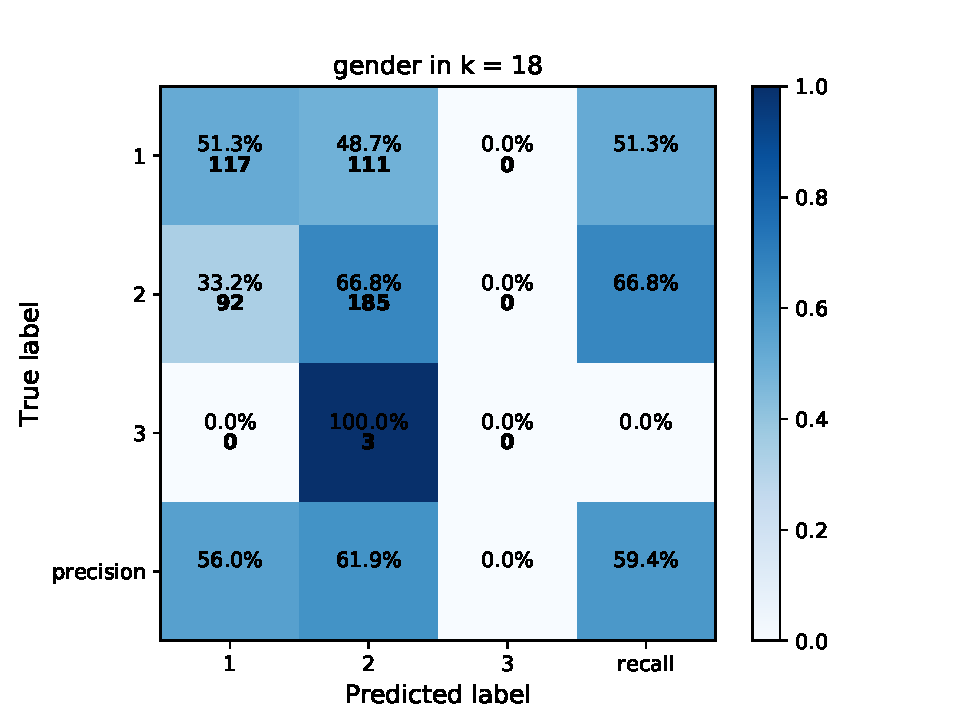
\includegraphics[scale=0.45]{fig/super_knn_gender.pdf}
    \end{subfigure}%
    \begin{subfigure}
      \centering
      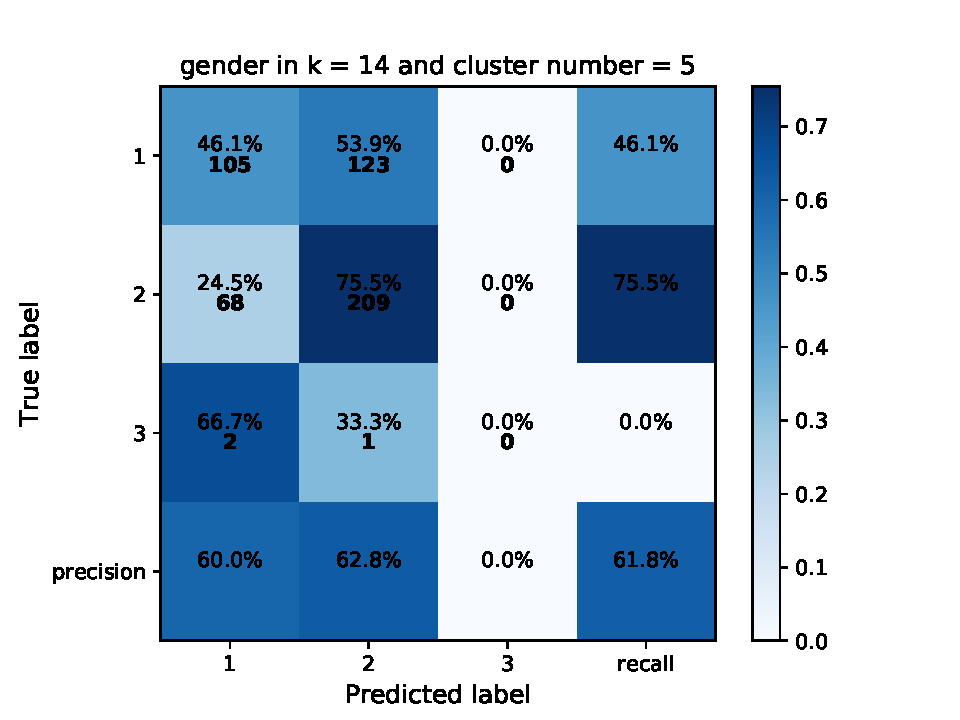
\includegraphics[scale=0.45]{fig/kms_knn_gender.pdf}
    \end{subfigure}
\end{figure*}

\begin{figure}[h]
    \centering
    \begin{subfigure}
      \centering
      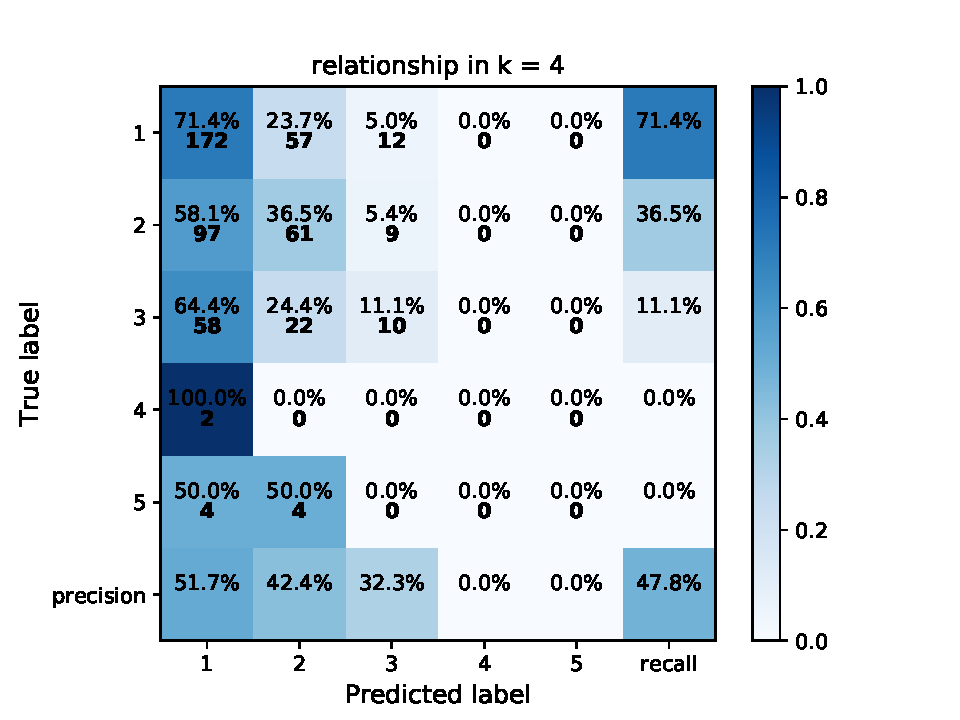
\includegraphics[scale=0.45]{fig/super_knn_relationship.pdf}
    \end{subfigure}%
    \begin{subfigure}
      \centering
      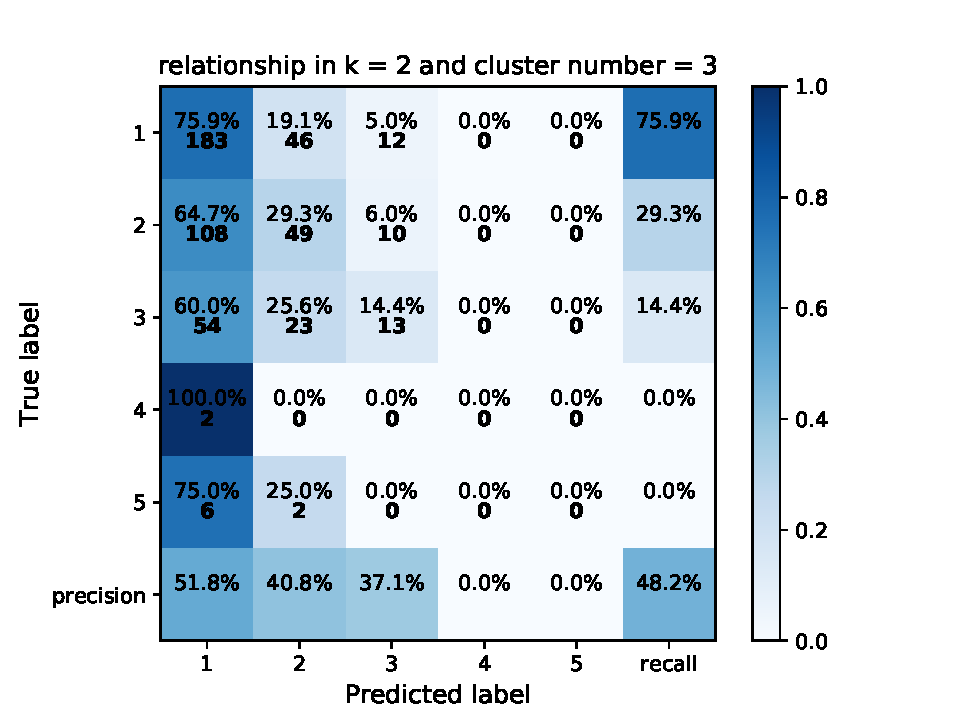
\includegraphics[scale=0.45]{fig/kms_knn_relationship.pdf}
    \end{subfigure}
    \caption{左側為 k-NN 預測個人資訊之混淆矩陣、右側為分群後以 k-NN 預測個人資訊之混淆矩陣}
    \label{fig:knn_con}
\end{figure}

\begin{figure*}[h]
    \centering
    \begin{subfigure}
      \centering
      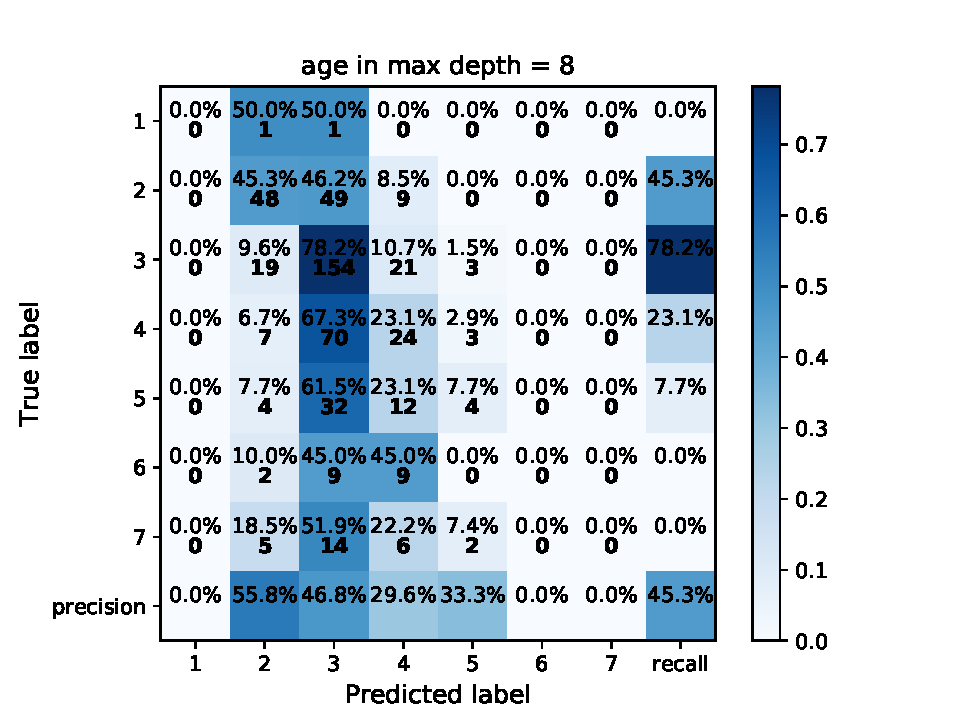
\includegraphics[scale=0.45]{fig/super_rf_age.pdf}
    \end{subfigure}%
    \begin{subfigure}
      \centering
      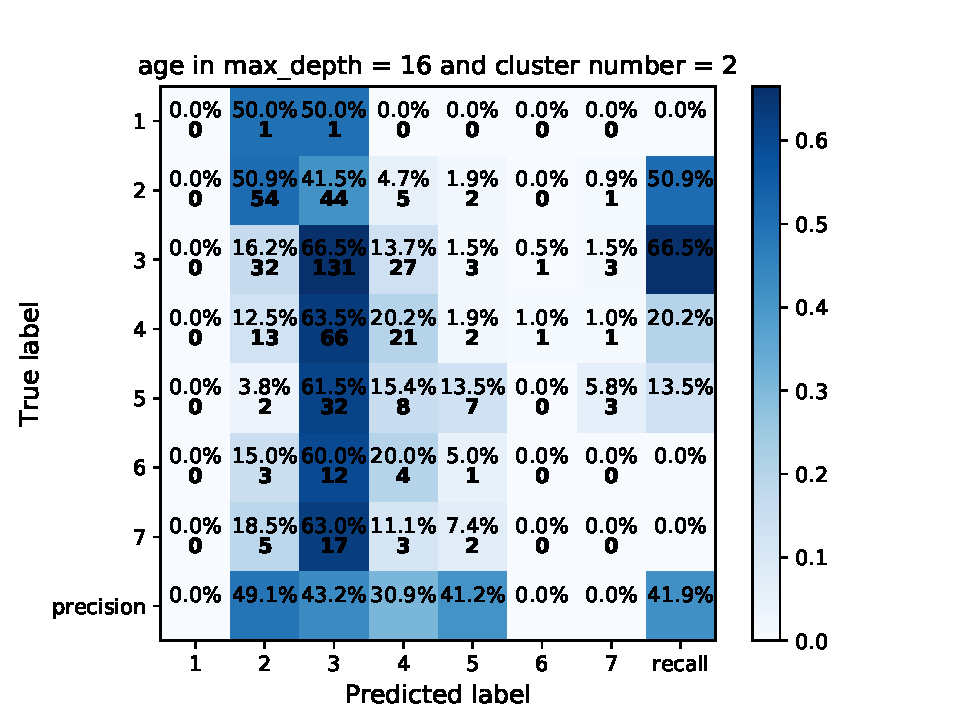
\includegraphics[scale=0.45]{fig/kms_rf_age.pdf}
    \end{subfigure}
\end{figure*}

\begin{figure*}[h]
    \centering
    \begin{subfigure}
      \centering
      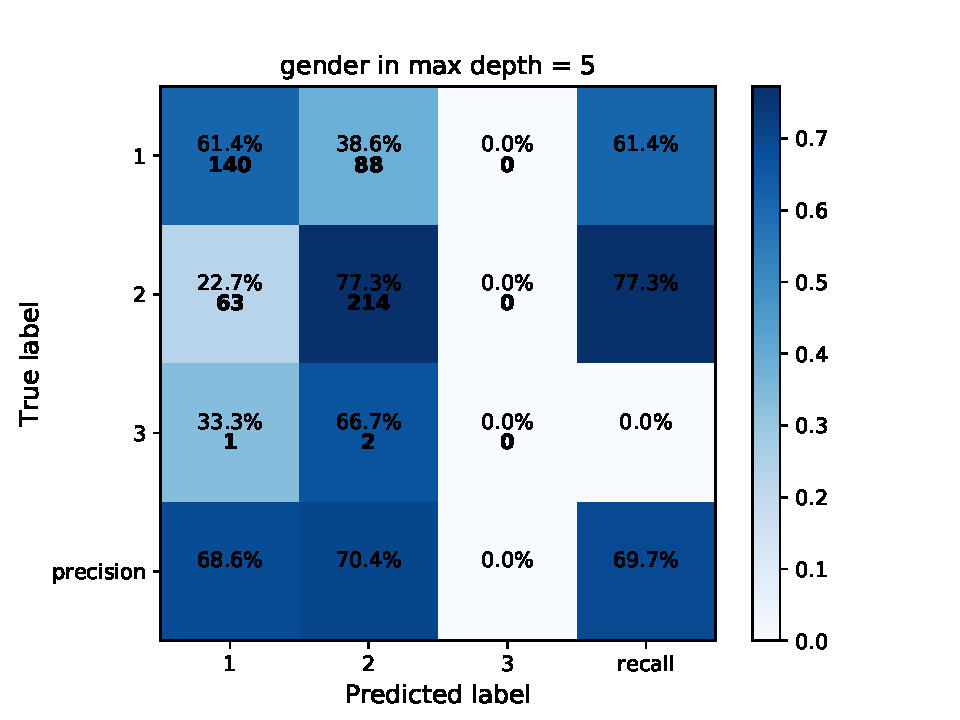
\includegraphics[scale=0.45]{fig/super_rf_gender.pdf}
    \end{subfigure}%
    \begin{subfigure}
      \centering
      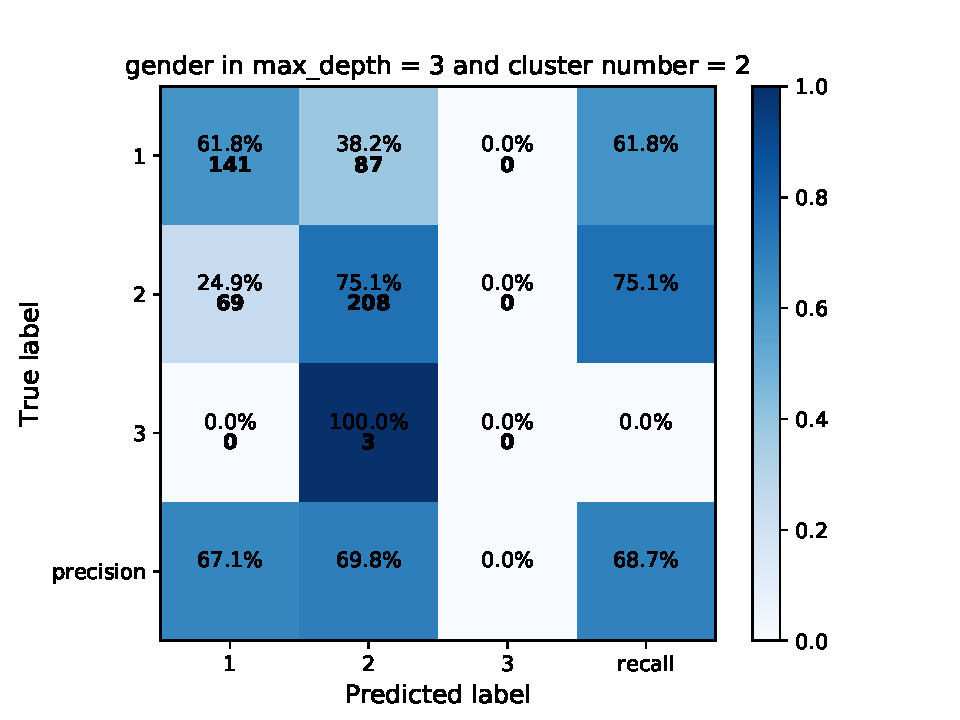
\includegraphics[scale=0.45]{fig/kms_rf_gender.pdf}
    \end{subfigure}
\end{figure*}

\begin{figure}[h]
    \centering
    \begin{subfigure}
      \centering
      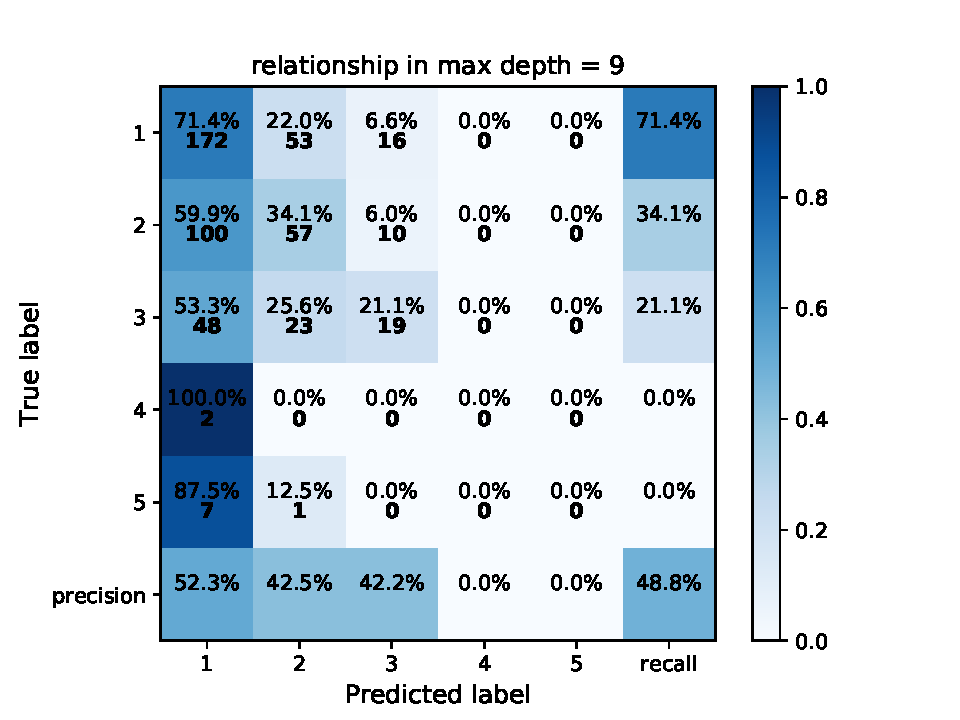
\includegraphics[scale=0.45]{fig/super_rf_relationship.pdf}
    \end{subfigure}%
    \begin{subfigure}
      \centering
      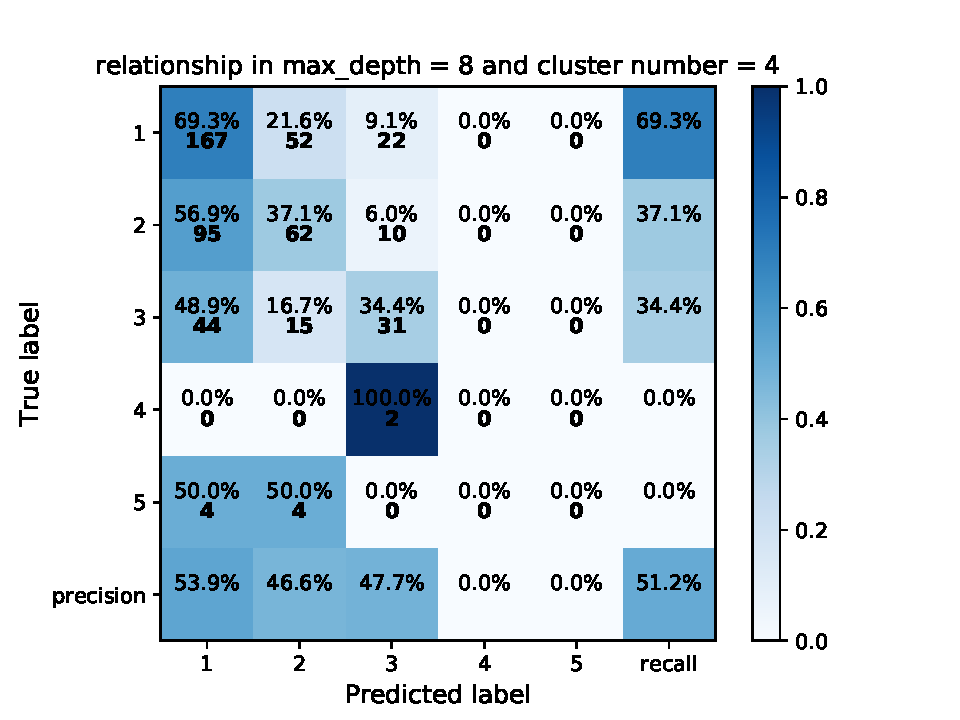
\includegraphics[scale=0.45]{fig/kms_rf_relationship.pdf}
    \end{subfigure}
    \caption{左側為 Random forests 預測個人資訊之混淆矩陣、右側為分群後以 Random forests 預測個人資訊之混淆矩陣}
    \label{fig:rf_con}
\end{figure}

\begin{figure*}[h]
    \centering
    \begin{subfigure}
      \centering
      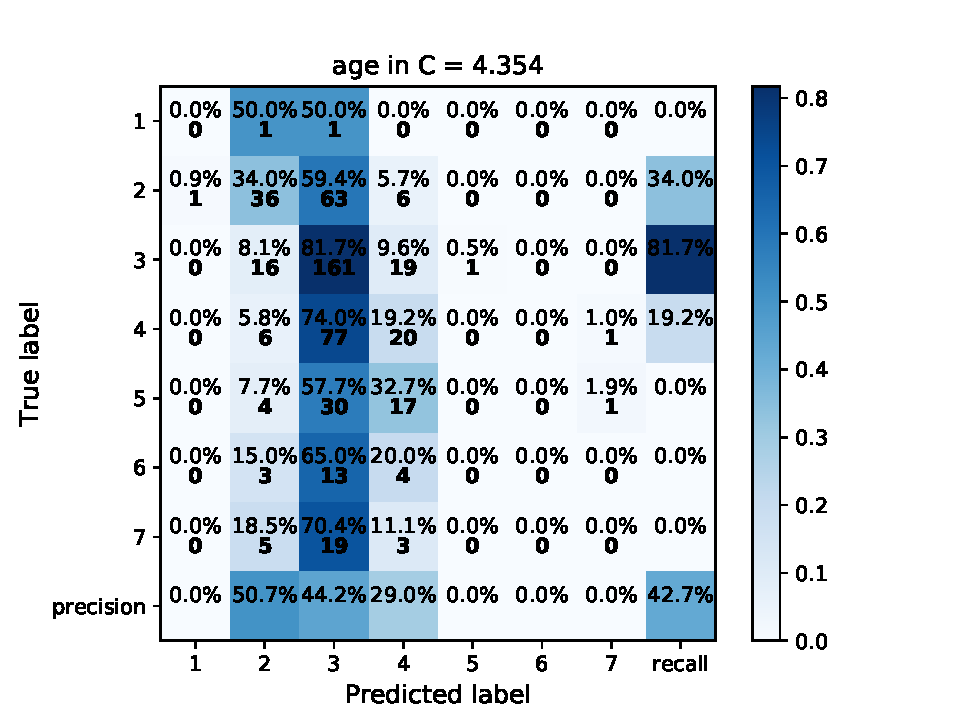
\includegraphics[scale=0.45]{fig/super_lr_age.pdf}
    \end{subfigure}%
    \begin{subfigure}
      \centering
      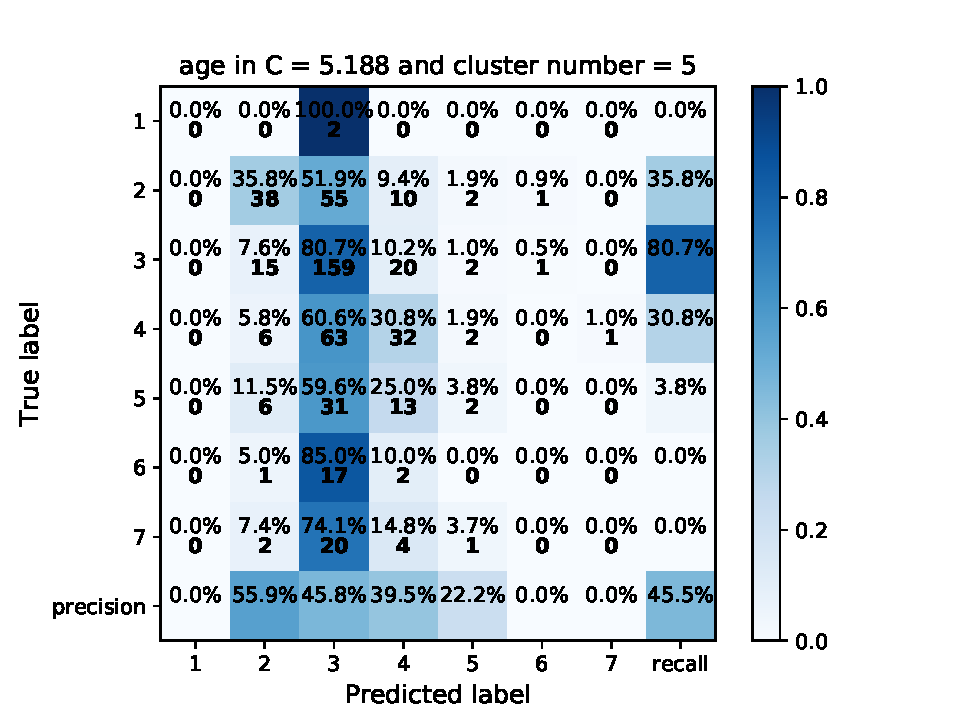
\includegraphics[scale=0.45]{fig/kms_lr_age.pdf}
    \end{subfigure}
\end{figure*}

\begin{figure*}[h]
    \centering
    \begin{subfigure}
      \centering
      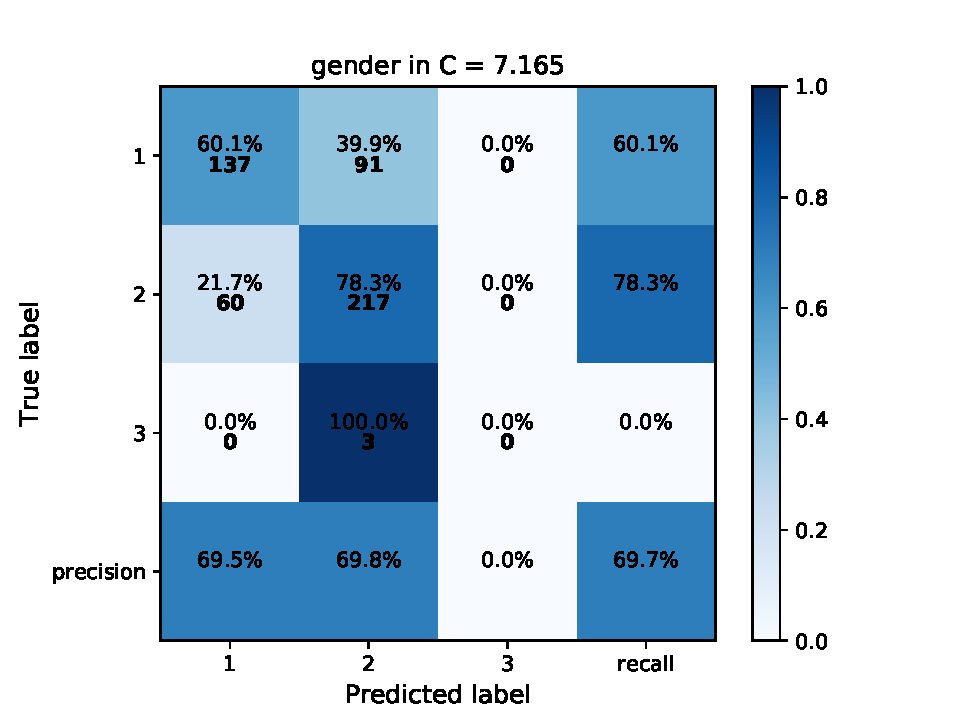
\includegraphics[scale=0.45]{fig/super_lr_gender.pdf}
    \end{subfigure}%
    \begin{subfigure}
      \centering
      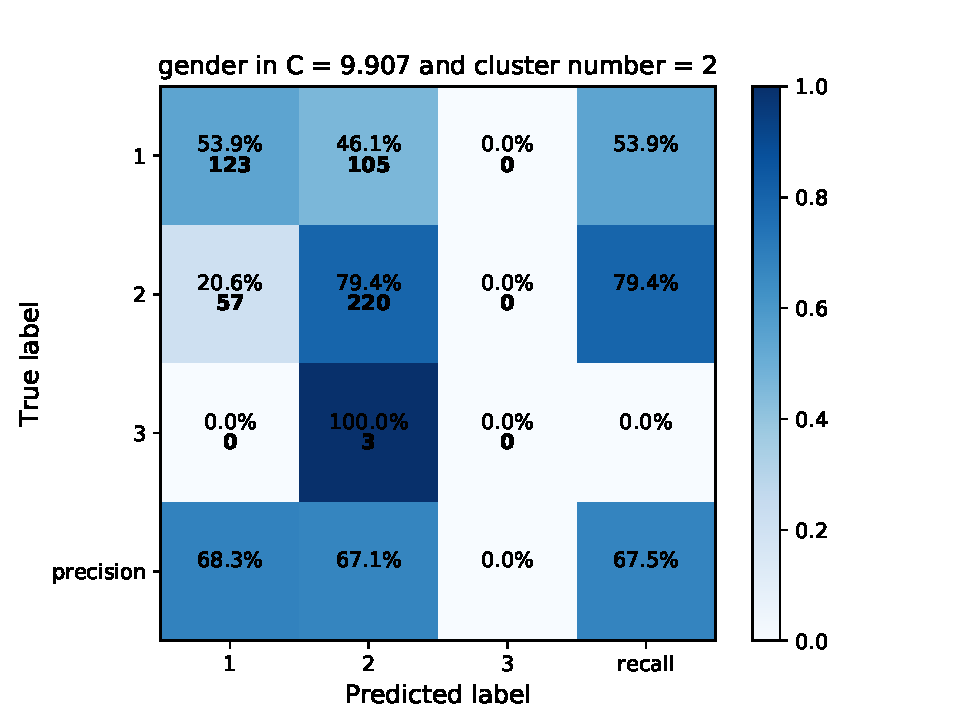
\includegraphics[scale=0.45]{fig/kms_lr_gender.pdf}
    \end{subfigure}
\end{figure*}

\begin{figure}[h]
    \centering
    \begin{subfigure}
      \centering
      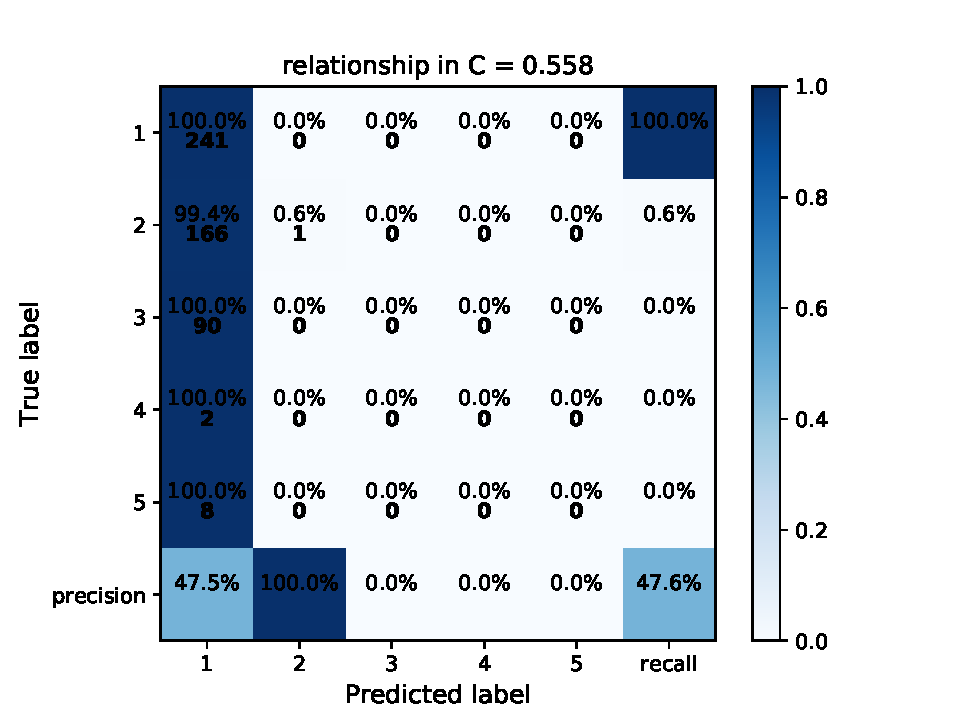
\includegraphics[scale=0.45]{fig/super_lr_relationship.pdf}
    \end{subfigure}%
    \begin{subfigure}
      \centering
      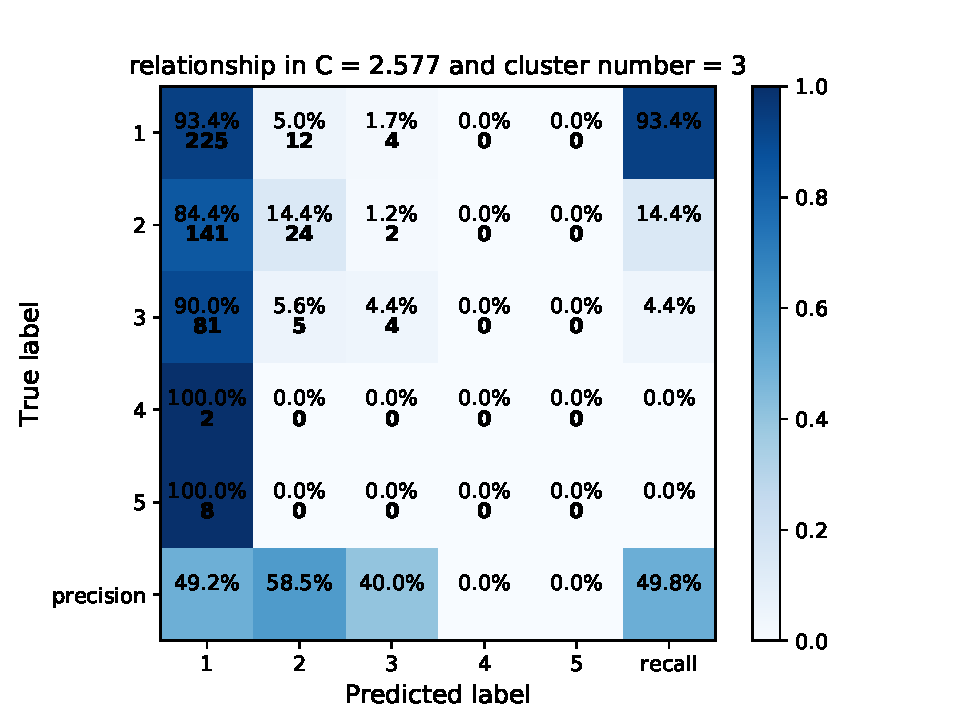
\includegraphics[scale=0.45]{fig/kms_lr_relationship.pdf}
    \end{subfigure}
    \caption{左側為 Logistic regression 預測個人資訊之混淆矩陣、右側為分群後以 Logistic regression 預測個人資訊之混淆矩陣}
    \label{fig:lr_con}
\end{figure}

\begin{figure*}[h]
    \centering
    \begin{subfigure}
      \centering
      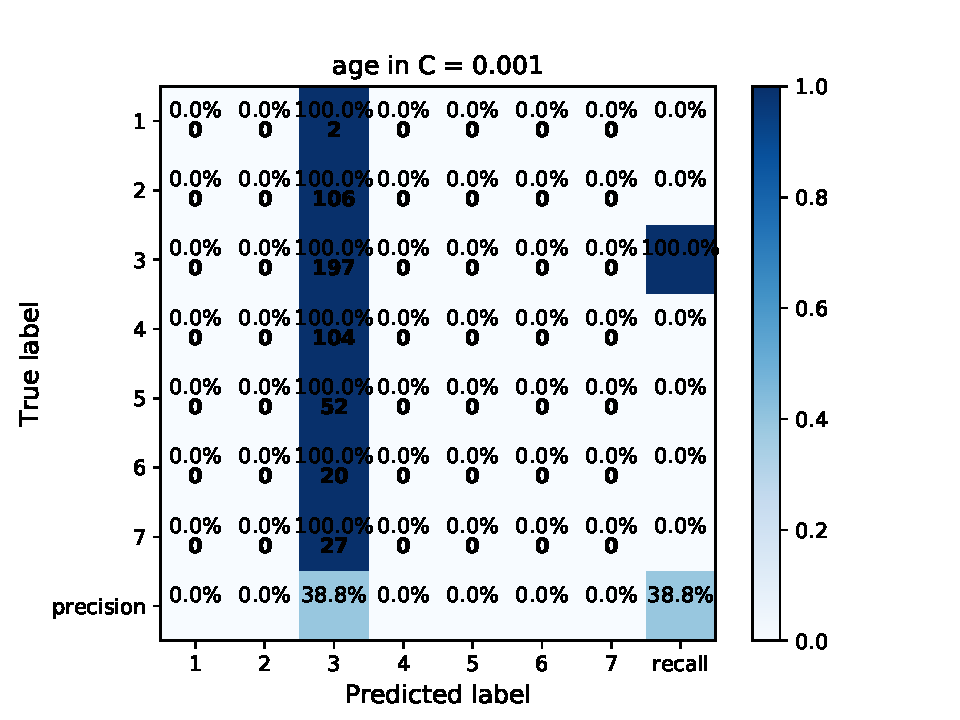
\includegraphics[scale=0.45]{fig/super_svm_age.pdf}
    \end{subfigure}%
    \begin{subfigure}
      \centering
      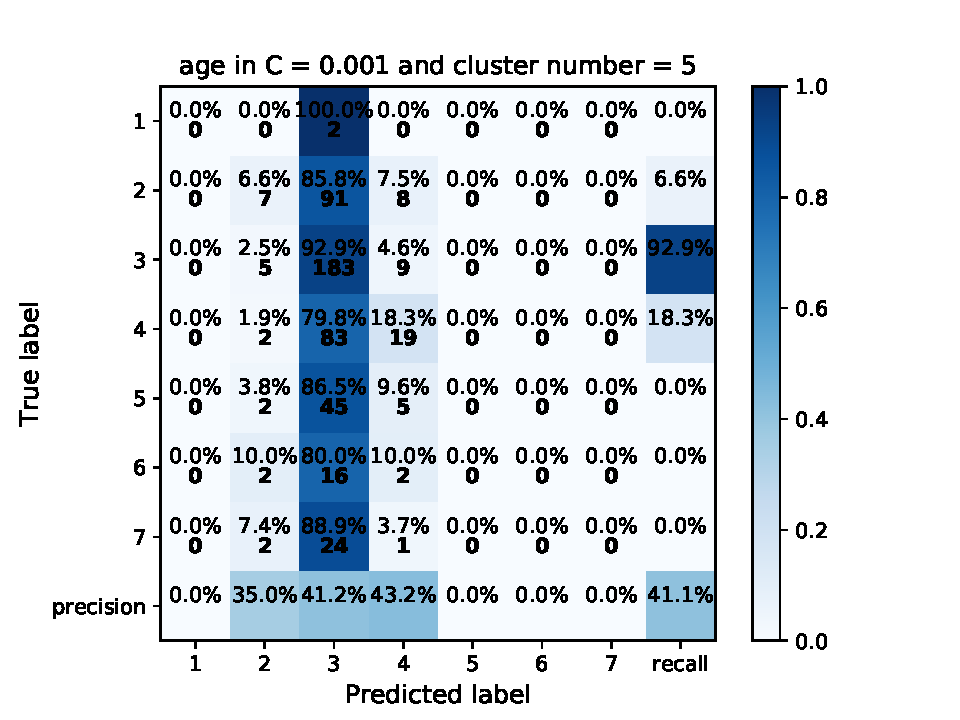
\includegraphics[scale=0.45]{fig/kms_svm_age.pdf}
    \end{subfigure}
\end{figure*}

\begin{figure*}[h]
    \centering
    \begin{subfigure}
      \centering
      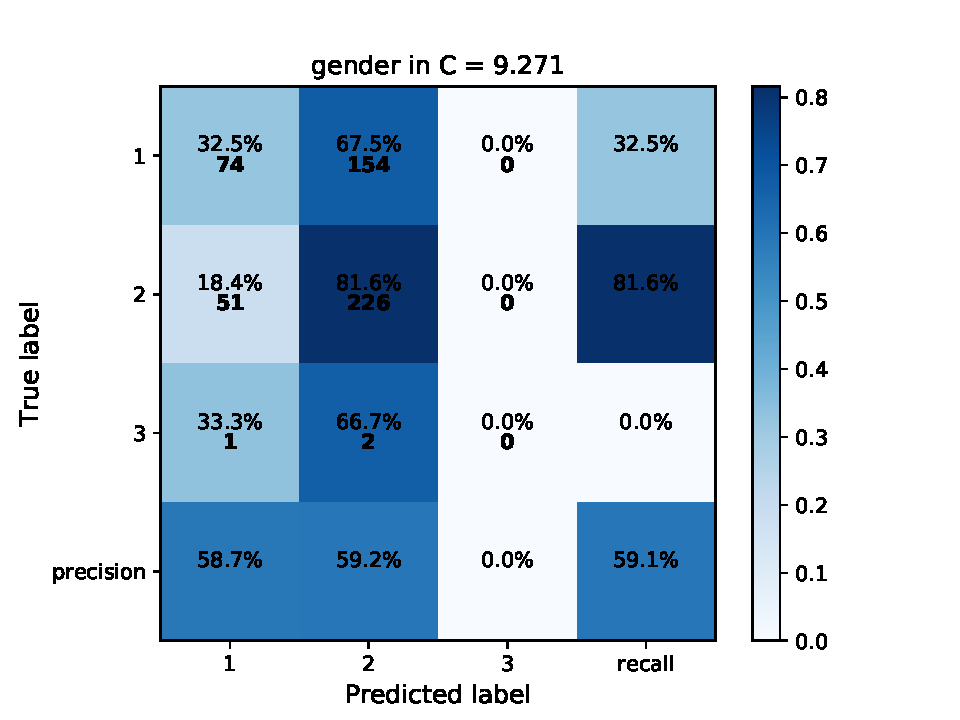
\includegraphics[scale=0.45]{fig/super_svm_gender.pdf}
    \end{subfigure}%
    \begin{subfigure}
      \centering
      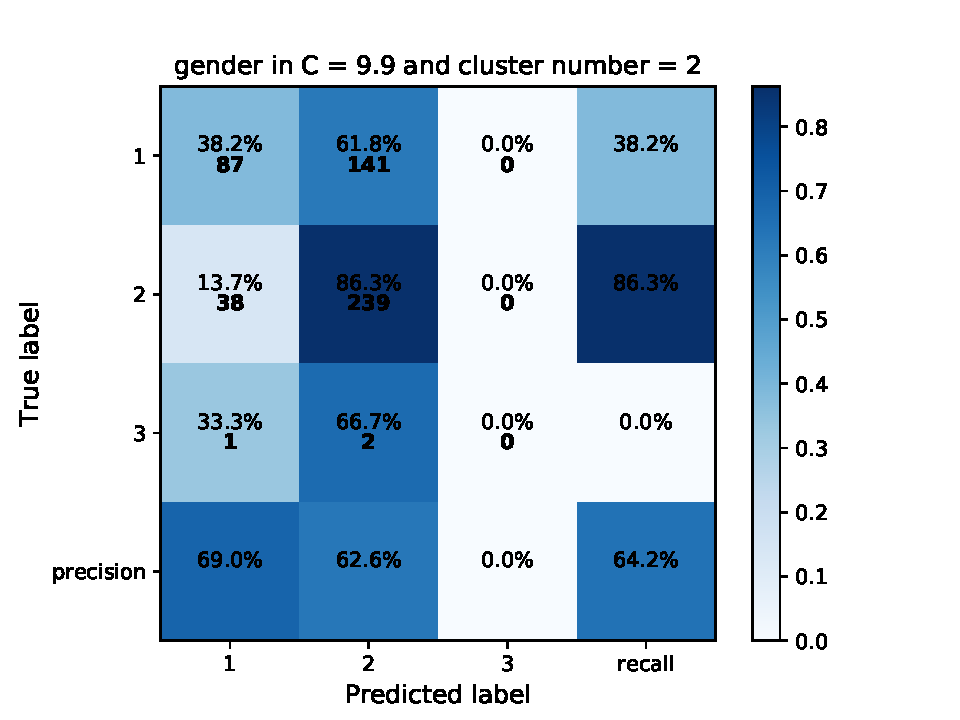
\includegraphics[scale=0.45]{fig/kms_svm_gender.pdf}
    \end{subfigure}
\end{figure*}

\begin{figure}[h]
    \centering
    \begin{subfigure}
      \centering
      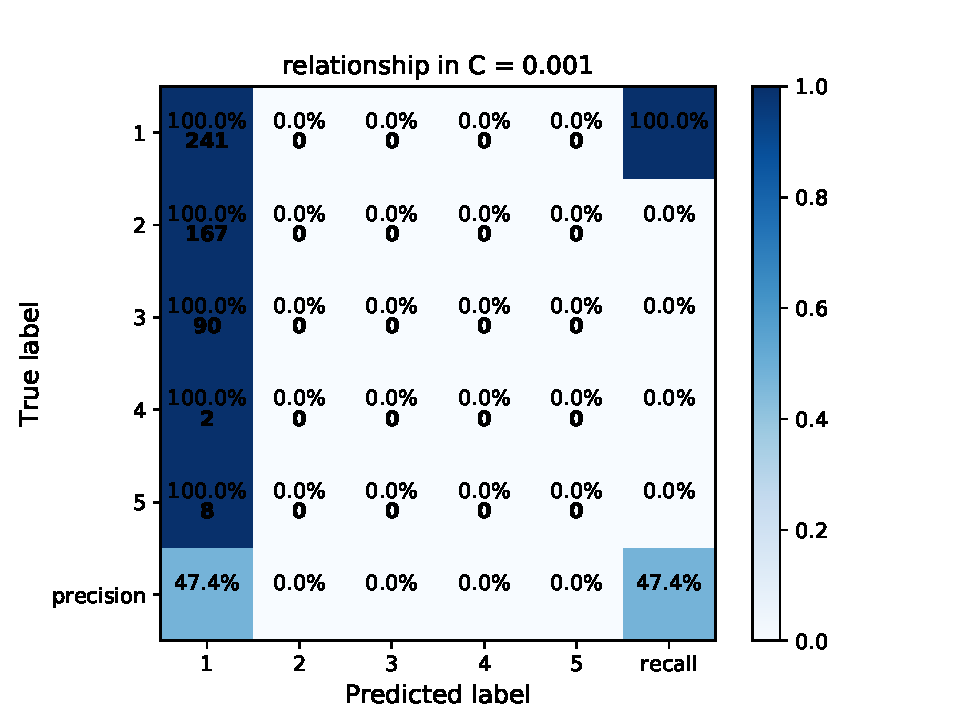
\includegraphics[scale=0.45]{fig/super_svm_relationship.pdf}
    \end{subfigure}%
    \begin{subfigure}
      \centering
      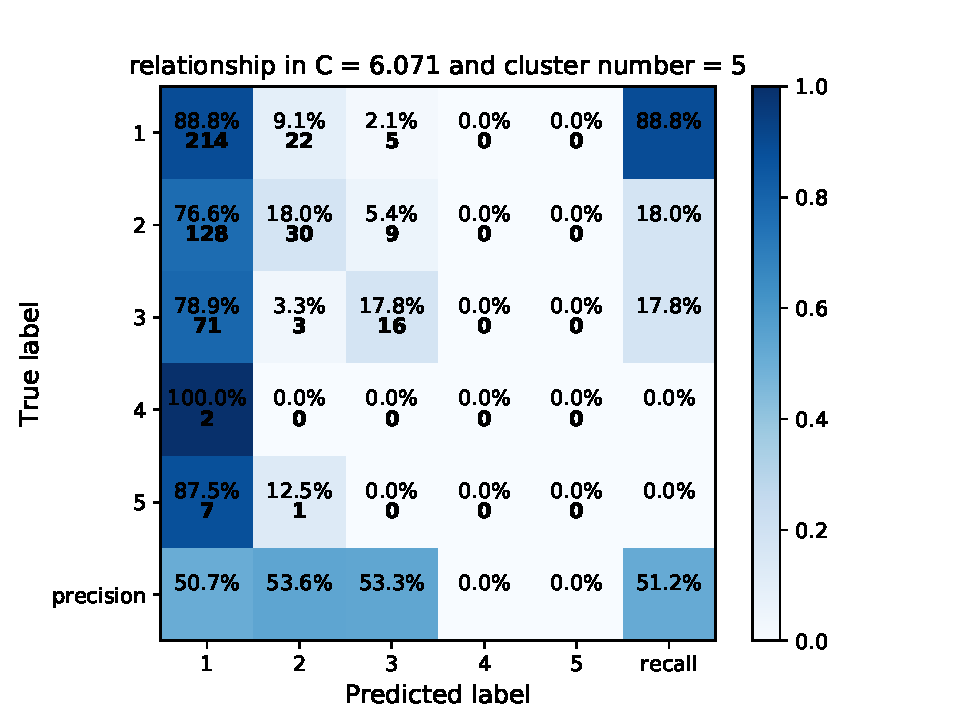
\includegraphics[scale=0.45]{fig/kms_svm_relationship.pdf}
    \end{subfigure}
    \caption{左側為 SVM 預測個人資訊之混淆矩陣、右側為分群後以 SVM 預測個人資訊之混淆矩陣}
    \label{fig:svm_con}
\end{figure}

}
\clearpage
\section{預測大六性格特質分數之結果比較}
{
本節將介紹以 $4$ 種方法:SVM、Lasso regression、Ridge regression 以及 Elastic net regression 之參數設定,並在最後以均方根誤差(root-mean-square error)比較 “基於監督式學習” 與 “結合分群之監督式學習” 兩者大六性格特質分數之預測結果。\par

基於監督式學習之預測方法中,使用 SVM 預測大六性格特質分數時能夠透過調整其中 regularization term 之權重($C$)來得到較低的 $RMSE$ 分數,其中盡責性(Conscientiousness)預測較準確($RMSE_{Con}=5.232$,$C=4.378$),而真誠性(Honesty-Humility)預測較差($RMSE_{HH}=5.789$,C=10)。而使用 Lasso regression、Ridge regression、Elastic net regression 預測大六性格特質分數時,同樣能透過調整 regularization term 之權重($Alpha$)來得到較佳的預測結果。Lasso regression 中預測盡責性(Conscientiousness)預測較準確($RMSE_{Con}=5.406$,$Alpha=0.001$),而外向性(Extraversion)預測較差($RMSE_{Ext}=5.881$,\\
$Alpha=0.001$)。Ridge regression 中預測盡責性(Conscientiousness)預測較準確($RMSE_{Con}=5.43$,$Alpha=0.001$),而情緒不穩定性(Neuroticism)預測較差($RMSE_{Neu}=5.981$,$Alpha=0.001$)。Elastic net regression 中預測盡責性(Conscientiousness)預測較準確($RMSE_{Con}=5.366$,$Alpha=0.001$),而真誠性(Honesty-Humility)預測較差($RMSE_{HH}=5.813$,$Alpha=0.001$)。詳細預測結果如表~\ref{tab:super_pr}。\par

\begin{table}[h]  
    \Large  
    \centering
    \fontsize{12}{20}\selectfont 
    \caption{基於監督式學習預測大六性格特質分數之結果}  
    \label{tab:super_pr}
    \begin{center}  
    \begin{tabular}{|l|l|l|l|l|}  
    \hline  
    Big-six personality& SVM & Lasso & Ridge & Elastic net \cr \hline  
    真誠性 & {\bf 5.789} & 5.832 & 5.845 & 5.813 \cr \hline  
    情緒不穩定性 & 5.78 & 5.87 & 5.981 & {\bf 5.769} \cr \hline 
    外向性 & 5.746 & 5.881 & 5.891 & {\bf 5.743} \cr \hline 
    親和性 & 5.643 & 5.71 & 5.795 & {\bf 5.622} \cr \hline 
    盡責性 & {\bf 5.232} & 5.406 & 5.43 & 5.366 \cr \hline 
    經驗開放性 & {\bf 5.38} & 5.607 & 5.646 & 5.44 \cr  
    \hline  
    \end{tabular}  
    \end{center}  
\end{table}  
\clearpage

結合分群之監督式學習的預測方法中,將使用者利用 k-means 將使用者分成 2 到 6 群後進行 SVM、Lasso regression、Ridge regression、Elastic net regression 進行大六性格特質分數之預測。使用 SVM 進行預測時,預測盡責性(Conscientiousness)預測較準確($RMSE_{Con}=5.048$,$C=9.353$,分群數$=4$),而情緒不穩定性(Neuroticism)預測較差($RMSE_{Neu}=5.623$,$C=9.53$,分群數$=4$)。使用 Lasso regression 進行預測時,預測盡責性(Conscientiousness)預測較準確($RMSE_{Con}=5.022$,$Alpha=0.245$,分群數$=4$),而情緒不穩定性(Neuroticism)預測較差($RMSE_{Neu}=5.469$,$Alpha=0.049$,分群數$=5$)。使用 Ridge regression 進行預測時,預測預測盡責性(Conscientiousness)預測較準確($RMSE_{Con}=5.027$,$Alpha=9.255$,分群數$=4$),而真誠性(Honesty-Humility)預測較差($RMSE_{HH}=5.43$,$Alpha=8.864$,分群數$=2$)。使用 Elastic net regression 進行預測時,預測盡責性(Conscientiousness)預測較準確($RMSE_{Con}=5.022$,$Alpha=0.398$,分群數$=4$),而外向性(Extraversion)預測較差($RMSE_{Ext}=5.422$,$Alpha=0.034$,分群數$=5$)。詳細預測結果如表~\ref{tab:kms_pr}。\par

\begin{table}[h]  
    \Large  
    \centering
    \fontsize{12}{20}\selectfont 
    \caption{結合分群之監督式學習預測大六性格特質分數結果}  
    \label{tab:kms_pr}
    \begin{center}  
    \begin{tabular}{|l|c|c|c|c|}  
    \hline  
    Big-six personality & SVM & Lasso & Ridge & Elastic net \cr \hline  
    真誠性 & 5.432 & {\bf 5.411} & 5.43 & 5.417 \cr \hline  
    情緒不穩定性 & 5.623 & 5.469 & 5.404 & {\bf 5.383} \cr \hline 
    外向性 & 5.402 & 5.435 & {\bf 5.38} & 5.422 \cr \hline 
    親和性 & 5.328 & 5.322 & 5.325 & {\bf 5.317} \cr \hline 
    盡責性 & 5.048 & {\bf 5.022} & 5.027 & {\bf 5.022} \cr \hline 
    經驗開放性 & 5.165 & 5.131 & {\bf 5.052} & 5.095 \cr  
    \hline  
    \end{tabular}  
    \end{center}  
\end{table} 
\clearpage

再透過比較 “將使用者分群後總是預測平均值(baseline)”、“基於監督式學習” 與 “結合分群之監督式學習” 大六性格特質分數之最佳預測結果(表~\ref{tab:total_pr}),可以了解結合分群之監督式學習之預測準確度在六種性格上皆高過基於監督式學習。

\begin{table}[h]  
    \Large  
    \centering
    \fontsize{12}{20}\selectfont 
    \caption{基於監督式學習與結合分群監督式學習之預測 $RMSE$ 分數比較表}  
    \label{tab:total_pr}
    \begin{center}  
    \begin{tabular}{|l|c|c|c|}  
    \hline  
    Big-six personality& Baseline & 基於監督式學習 & 結合分群監督式學習 \cr \hline  
    真誠性 & 5.806 & 5.789 & {\bf 5.411} \cr \hline  
    情緒不穩定性 & 5.718 & 5.769 & {\bf 5.383} \cr \hline 
    外向性 & 5.721 & 5.743 & {\bf 5.38} \cr \hline 
    親和性 & 5.604 & 5.622 & {\bf 5.317} \cr \hline 
    盡責性 & 5.224 & 5.232 & {\bf 5.022} \cr \hline 
    經驗開放性 & 5.281 & 5.38 & {\bf 5.052} \cr  
    \hline  
    \end{tabular}  
    \end{center}  
\end{table} 
}

\section{實驗結果分析}
\subsection{預測個人資訊結果分析}
{
k-NN 對於年齡方面的預測(圖~\ref{fig:knn_con} 中 age 部分),分群結果對於 $26\sim30$ 歲(Label:3)的使用者族群能夠更加準確被分類出來,但是對於 $21\sim25$ 歲(Label:2)的族群預測準確度明顯下降。性別方面相較年齡之預測效果更加成功,分群後預測準確度是 3 種個人資訊中效果提升最多的項目。而感情狀態中分群對於準確度幫助較少。\par

Random forests 對於年齡方面預測(圖~\ref{fig:rf_con} 中 age 部分)是 4 種分類器中效果最好的,但是分群後的準確度反而下降許多,但是對於 $21\sim25$ 歲(Label:2)的族群更能夠分類正確。性別方面(圖~\ref{fig:rf_con} 中 gender 部分),分群後對於女性(Label:2)分類效果較差,因此分群後反而整體準確度下降。而感情狀態(圖~\ref{fig:rf_con} 中 relationship 部分)中分群對於已婚(Label:3)的使用者能夠更加正確分類出來,因此整體預測效果上升許多。\par

Logistic regression 對於年齡方面的預測(圖~\ref{fig:lr_con} 中 age 部分)較於偏向分類為 $26\sim30$ 歲(Label:3),但是其中對於 $21\sim25$ 歲(Label:2)的族群反而是 4 種分類器中準確度最高的。性別方面(圖~\ref{fig:lr_con} 中 gender 部分)與 Random forests 類似,也是屬於分群後準確度降低的類型。而感情狀態方面(圖~\ref{fig:lr_con} 中 relationship 部分),總是預測使用者為單身(Label:1),而分群後由於訓練集中已婚(Label:3)的使用者所佔比例提升,因此對於已婚的使用者較能夠分類出來,所以整體準確度上升。\par

SVM 與 Logistic regression 預測結果有點類似,個人資訊中各方面都偏向預測樣本數最多的種類,而分群後較能夠預測出部分樣本數較少的使用者類別。由於偏向猜測樣本數最多的種類,因此與 baseline 預測分數較為類似。其中性別方面(圖~\ref{fig:svm_con} 中 gender 部分),分類器比較有學到正確的分類方式,因此預測結果比 baseline 高出許多。\par

綜合以上結果,分群對於感情狀態的分類效果比較幫助,4 種分類器經過分群準確度都有上升。而性別方面,預測準確度最高的為直接以 Random forests 與 Logistic regression 進行預測,而分群後之預測準確度反而下降,與原本預期中的結果不太相同。
}

\subsection{預測大六性格特質分數結果分析}
{
大六性格特質分數之預測中,SVM、Lasso、Ridge、Elastic net regression 之預測表現皆為結合分群的預測結果較好,其中 Lasso、Ridge、Elastic net regression 在分群之前對於 regularization term 都給予很小的權重,幾乎傾向做 regularization,但是在分群後則都對 regularization term 給予了不同的權重,表示分群對於使用線性回歸之預測有很大的幫助,而在最後的結果比較方面,也能夠明顯看出結合分群之效能有明顯提升。\par

其中比較特別的部分為 SVM 在未結合分群的狀態下,預測效果在真誠性、盡責性、經驗開放性是優於其他 3 種回歸方法的,而在結合分群之後 6 種性格特質分數中並沒有特別突出的表現,目前還找不到明確原因來解釋此現象。
}
\chapter{結論與未來展望}
\section{結論}
{
本篇論文之實驗結果,主要分為預測使用者個人資訊以及預測使用者之大六性格特質分數兩個部分。當預測個人資訊時,使用結合分群監督式學習的預測方法在類別數量較多(年齡、感情狀態)的預測較為準確,但相對於基於監督式學習之預測方法並沒有太大的提升,其中使用 Random forests 作為分類器的效能是相對高的。使用者特徵中,使用者於各類型網頁之瀏覽比例對於預測年齡與性別影響度較高,使用者於一天中各時段之瀏覽比例對於感情狀態之預測的影響度較高。\par

預測大六性格特質分數時,利用結合分群監督式學習的預測準確度皆高於基於監督式學習,使用 Lasso、Ridge、Elastic net regression 在預測各項分數時皆有不同的優勢。大六性格特質分數中真誠性與情緒不穩定性較難以預測,而盡責性在四種回歸模型上都有良好的預測效果。使用者特徵中,使用者於各類型網頁之瀏覽比例對於大部分的性格特質分數影響度較高,而使用者於一天中各時段之瀏覽比例對於親和性之預測的影響度較高。\par

本篇論文對於藉由使用者之網頁瀏覽紀錄進行個人資訊與六大性格特質分數之預測皆有良好的效能展現,對於使用者個人資訊難以取得之問題做出改善,並且對於使用者個性特質能夠具有一定程度的了解。基於此研究成果,對於心理學研究方面,使得大六性格特質分數添加了更多的參考層面。以往的大六性格特質分數是藉由使用者對特定問題之回答來推估各項特質分數,現在更能夠透過本篇論文之預測方法,增進大六性格特質分數計算準確度。若擁有使用者之網頁瀏覽紀錄資訊,對於使用者相關資訊之研究,則不再侷限於個人資訊的預測,而是能夠更加深入了解使用者的個性,並拓展了使用者行為分析的視野。
}
\clearpage

\section{未來展望}
{
由於本實驗使用的資料集中使用者人數較少(672 人),因此在進行測試集預測時,容易受到其中幾位使用者之預測錯誤導致整體預測分數過低。若未來能夠蒐集更多使用者的網頁瀏覽紀錄與其個人詳細資訊,對於機器學習將會有很大的幫助,也能夠提升預測之準確率。\par

對於預測個人資訊與大六性格特質分數所使用的分類器與分群數量多寡,若能夠找出其之間的相關性將能夠大幅提升預測效能與降低實驗所需時間,因此未來將會朝向這方面找出解決方法。\par

另一方面,若使用者人數增加到一定足夠的量,將能夠結合深度學習。由於使用者之網頁瀏覽紀錄具有時序性特徵,結合長短期記憶(LSTM~\cite{hochreiter1997long})結構之類神經網路進行預測,將能夠在相對的節日對使用者之個人資訊得到更準確的預測,例如:聖誕節前夕,對於餐廳、約會類別的網頁瀏覽率將會影響其感情狀態之預測。\par


}
                                 % \backmatter

%\cleardoublepage                         % 保證奇數頁為章節起始
%\phantomsection
%\addcontentsline{toc}{chapter}{索引}     % 將索引加入目錄中

%\printindex

%\cleardoublepage                         % 保證奇數頁為章節起始
%\phantomsection
\addcontentsline{toc}{chapter}{參考文獻}     % 將參考文獻加入目錄中

\bibliographystyle{IEEEtran}      
\bibliography{myfoo}                   % 或標準資料庫用法          


                  % 文獻      (自行寫入)
\stepcounter{chapter} % This is trick to keep the bookmark correct
\begin{appendA}
\begin{alwayssingle}
 \\
 \\

實驗資料集:https://github.com/littlelienpeanut/DART\_predicting\_users\_demo/tree/master/dataset \par

實驗程式碼:https://github.com/littlelienpeanut/DART\_predicting\_users\_demo\par

實驗步驟:\par
\begin{center}
\begin{enumerate}

\item 透過 user\_daily.py (v4、v5)對原始資料進行前處理,生成第三章所介紹的兩種使用者特徵資料。
\item 利用 supervise\_demo.py 進行不同監督式學習方法之使用者個人資訊預測。
\item 利用 supervise\_pr.py 進行不同監督式學習方法之使用者大六人格分數預測。
\item 利用 kms\_demo.py 進行不同分群結合監督式學習方法之使用者個人資訊預測。
\item 利用 kms\_pr.py 進行不同分群結合監督式學習方法之使用者大六人格分數預測。
\end{enumerate}
\end{center} \par
實驗詳細步驟將在實驗程式碼之網址上敘述。
\end{alwayssingle}
\end{appendA}               % 若有需要 使用appendA/B環境
 

\end{CJK}                        
%---------------------
%\clearpage
%\bookbone                        % 短書脊製作
%{\centering\layout}
\end{document}                   % 本文結束
